\documentclass[10pt,twocolumn,letterpaper]{article}

% --- Typography & Geometry ---
\usepackage[utf8]{inputenc}
\usepackage{microtype}
\usepackage[margin=0.75in,top=0.85in,bottom=0.85in]{geometry}

% --- Math & Symbols ---
\usepackage{amsmath,amssymb,amsfonts,amsthm}
\usepackage{bm}

% --- Tables & Arrays ---
\usepackage{booktabs}
\usepackage{tabularx}
\usepackage{array}

% --- Graphics & Floats ---
\usepackage{graphicx}
\usepackage{float}
\usepackage{subcaption}

% --- Code Listings ---
\usepackage{xcolor}
\usepackage{listings}

\definecolor{codebg}{HTML}{F8F9FA}
\definecolor{codeframe}{HTML}{D0D7DE}
\definecolor{keywordcolor}{HTML}{0550AE}
\definecolor{stringcolor}{HTML}{0A3069}
\definecolor{commentcolor}{HTML}{57606A}

\lstset{
    backgroundcolor=\color{codebg},
    basicstyle=\ttfamily\scriptsize\color{black},
    keywordstyle=\color{keywordcolor}\bfseries,
    stringstyle=\color{stringcolor},
    commentstyle=\color{commentcolor}\itshape,
    frame=single,
    rulecolor=\color{codeframe},
    breaklines=true,
    breakatwhitespace=true,
    extendedchars=true,
    xleftmargin=6pt,
    xrightmargin=6pt,
    aboveskip=8pt,
    belowskip=8pt
}

% --- Hyperlinks ---
\usepackage{hyperref}
\hypersetup{
    colorlinks=true,
    linkcolor=blue!70!black,
    citecolor=blue!70!black,
    urlcolor=blue!70!black
}

% --- Input Title & Authors ---

\section{Primal Attention: Self-Attention via Asymmetric Kernel SVD in Primal Representation}


\textbf{Authors:}
\begin{itemize}
\item {{AUTHOR\_1\_NAME}}  -- {{AUTHOR\_1\_EMAIL}}
\end{itemize}
\begin{itemize}
\item {{AUTHOR\_2\_NAME}}  -- {{AUTHOR\_2\_EMAIL}}
\end{itemize}

\textbf{Affiliations:}
\begin{itemize}
\item   {{UNIVERSITY\_1}}, {{DEPARTMENT\_1}}
\end{itemize}
\begin{itemize}
\item   {{UNIVERSITY\_2}}, {{DEPARTMENT\_2}}
\end{itemize}

\textbf{Corresponding author:} {{CORRESPONDING\_AUTHOR}}
\textbf{Preprint date:} {{DATE}}
\textbf{Version:} v{{VERSION}}
\textbf{Code:} https://github.com/{{ORG}}/SVD\_Project/tree/main/framework/attentions/primal\_attention.py
\textbf{Model weights:} https://huggingface.co/{{HF\_ORG}}
\textbf{License:} {{LICENSE}}



\subsection{Abstract}

Standard softmax attention incurs $\mathcal{O}(L^2)$ time and memory in sequence 
length $L$, which becomes the bottleneck for long-context transformer inference. 
Nystr m approximation reduces this to $\mathcal{O}(L m)$ by projecting onto $m$ 
landmarks, but requires a symmetric kernel matrix, forcing the same landmarks 
for queries and keys. This is unnecessarily restrictive.

We introduce \textbf{Primal Attention}, an asymmetric kernel SVD formulation that 
decomposes the attention matrix as $A \approx F_1 F_2^{-1} F_3$, where $F_1, F_3$ 
are query-key cross products with landmarks and $F_2$ is the landmark-landmark 
Gram matrix. This allows independent landmark selection for queries and keys. 
The pseudoinverse $F_2^{-1}$ is computed via an iterative Schulz refinement 
that converges in a few steps and is differentiable.

Primal Attention selects landmarks via \textbf{segment pooling} over contiguous chunks 
of the sequence, providing a uniform but content-agnostic summary of the 
attention input. We evaluate on DistilBERT, RoBERTa-base, and GPT-2 on SST-2 
with landmark count $m = {{RANK}}$. Primal Attention achieves 
\textbf{{{D\_ACC}}\%}, \textbf{{{R\_ACC}}\%}, and \textbf{{{G\_ACC}}\%} accuracy respectively, 
at the cost of \textbf{{{D\_TIME\_RATIO}}$\times$} inference latency. The attention matrix 
memory is reduced by \textbf{{{MEM\_REDUCTION}}$\times$}. We provide a production-hardened 
PyTorch implementation supporting flat, nested, and causal architectures with 
GQA, RoPE, and safe injection.

\textbf{Keywords:} Nystr m approximation, low-rank attention, pseudoinverse, Schulz 
iteration, efficient transformer



\subsection{Lay Summary}

Attention is the core mechanism in modern language models. Its cost grows 
quadratically with sentence length -- doubling the input quadruples the work. 
Many methods try to reduce this by summarizing the input into a few "landmark" 
points, but these methods typically require the same landmarks for both the 
query and the key side.

Primal Attention breaks this symmetry: queries and keys can use different 
landmarks. This gives more flexibility and slightly better quality at the 
same cost. We test the method on three popular language models and find that 
it retains most of the original accuracy while reducing attention memory by 
a factor of several. The method is fully differentiable and integrates 
cleanly with existing pretrained models.



\subsection{Table of Contents}

1. [Introduction](01\_intro.md)
2. [Related Work](02\_related.md)
3. [Background](03\_background.md)
4. [Method](04\_method.md)
5. [Architecture Integration](05\_architecture.md)
6. [Experimental Setup](06\_setup.md)
7. [Results](07\_results.md)
8. [Analysis](08\_analysis.md)
9. [Discussion](09\_discussion.md)
10. [Limitations](10\_limitations.md)
11. [Conclusion](11\_conclusion.md)
12. [Reproducibility](12\_reproducibility.md)
13. [References](13\_references.md)

\textbf{Appendices:}
\begin{itemize}
\item [A. Mathematical Derivations](A\_math.md)
\end{itemize}
\begin{itemize}
\item [B. Implementation Details](B\_implementation.md)
\end{itemize}
\begin{itemize}
\item [C. Full Experimental Data](C\_data.md)
\end{itemize}
\begin{itemize}
\item [D. Negative Results](D\_negative\_results.md)
\end{itemize}
\begin{itemize}
\item [E. Ethical Considerations](E\_ethics.md)
\end{itemize}

\begin{document}

\maketitle

% --- Abstract & Keywords Block ---
\begin{abstract}
Standard softmax attention incurs $\mathcal{O}(L^2)$ time and memory in sequence 
length $L$, which becomes the bottleneck for long-context transformer inference. 
Nystr m approximation reduces this to $\mathcal{O}(L m)$ by projecting onto $m$ 
landmarks, but requires a symmetric kernel matrix, forcing the same landmarks 
for queries and keys. This is unnecessarily restrictive.

We introduce \textbf{Primal Attention}, an asymmetric kernel SVD formulation that 
decomposes the attention matrix as $A \approx F_1 F_2^{-1} F_3$, where $F_1, F_3$ 
are query-key cross products with landmarks and $F_2$ is the landmark-landmark 
Gram matrix. This allows independent landmark selection for queries and keys. 
The pseudoinverse $F_2^{-1}$ is computed via an iterative Schulz refinement 
that converges in a few steps and is differentiable.

Primal Attention selects landmarks via \textbf{segment pooling} over contiguous chunks 
of the sequence, providing a uniform but content-agnostic summary of the 
attention input. We evaluate on DistilBERT, RoBERTa-base, and GPT-2 on SST-2 
with landmark count $m = 64$. Primal Attention achieves 
\textbf{{{D\_ACC}}\%}, \textbf{{{R\_ACC}}\%}, and \textbf{{{G\_ACC}}\%} accuracy respectively, 
at the cost of \textbf{{{D\_TIME\_RATIO}}$\times$} inference latency. The attention matrix 
memory is reduced by \textbf{{{MEM\_REDUCTION}}$\times$}. We provide a production-hardened 
PyTorch implementation supporting flat, nested, and causal architectures with 
GQA, RoPE, and safe injection.

\textbf{Keywords:} Nystr m approximation, low-rank attention, pseudoinverse, Schulz 
iteration, efficient transformer



\vspace{0.5em}
\noindent\textbf{Keywords:} Nystr m approximation, low-rank attention, pseudoinverse, Schulz
\end{abstract}

\vspace{1em}

% --- Paper Body ---

\section{1. Introduction}

\subsection{1.1 Motivation}

The softmax attention mechanism (Vaswani et al., 2017) scales quadratically 
with sequence length $L$:

\[
\text{Attn}(Q, K, V) = \text{softmax}\!\left(\frac{Q K^\top}{\sqrt{d_h}}\right) V
\tag{1.1}
\]

producing an $L \times L$ attention matrix that requires $\mathcal{O}(L^2)$ 
memory and time. For a sequence of 4096 tokens at 12 heads, the attention 
matrix alone occupies \textbf{200 MB at FP16}, dwarfing the model's own weight 
footprint.

\textbf{Low-rank approximation} reduces this to $\mathcal{O}(L m)$ by projecting 
onto $m \ll L$ landmarks. The Nystr m method (Williams \& Seeger, 2001) does 
this by:

\[
K \approx \tilde{K} = C W^{-1} C^\top
\tag{1.2}
\]

where $C \in \mathbb{R}^{L \times m}$ is the query-landmark kernel and 
$W \in \mathbb{R}^{m \times m}$ is the landmark-landmark kernel. The 
Nystr mformer (Xiong et al., 2021) applies this to attention.

\textbf{The problem with standard Nystr m.} It assumes a symmetric kernel, 
requiring the same landmarks for queries and keys. In attention, however, 
queries and keys play different roles: queries ask "what am I looking for?"; 
keys answer "what am I?" Using the same landmarks ignores this asymmetry.

\subsection{1.2 Problem Statement}

Given query $Q \in \mathbb{R}^{L \times d}$, key $K \in \mathbb{R}^{L \times d}$, 
and value $V \in \mathbb{R}^{L \times d}$, we seek a low-rank approximation 
of the attention output:

\[
\text{Attn}(Q, K, V) \approx \text{Attn}_\text{low-rank}(Q, K, V)
\tag{1.3}
\]

such that:

1. \textbf{Complexity:} $\mathcal{O}(L m)$ instead of $\mathcal{O}(L^2)$, with $m \ll L$.
2. \textbf{Asymmetry:} Independent landmark selection for $Q$ and $K$.
3. \textbf{Differentiability:} End-to-end training.
4. \textbf{Compatibility:} Works with pretrained models without retraining.
5. \textbf{Stability:} Numerically robust for FP16 and long sequences.

\subsection{1.3 Our Approach: Primal Attention}

We propose \textbf{Primal Attention}, which decomposes the attention matrix 
asymmetrically:

\[
A \approx F_1 F_2^{-1} F_3
\tag{1.4}
\]

where:

\begin{itemize}
\item $F_1 = Q K_\text{land}^\top \in \mathbb{R}^{L \times m}$: query vs landmark keys
\item $F_2 = Q_\text{land} K_\text{land}^\top \in \mathbb{R}^{m \times m}$: landmark-landmark
\item $F_3 = Q_\text{land} K^\top \in \mathbb{R}^{m \times L}$: landmark queries vs keys
\end{itemize}

This is the \textbf{primal representation} of the asymmetric kernel (in contrast 
to the dual representation which uses $L \times L$ kernels). The pseudoinverse 
$F_2^{-1}$ is computed via \textbf{Schulz iteration}:

\[
X_{t+1} = X_t (2I - F_2 X_t)
\tag{1.5}
\]

which converges quadratically to $F_2^{-1}$ in a few steps and is differentiable.

\textbf{Landmark selection.} We use \textbf{segment pooling}: divide the sequence into 
$m$ equal chunks and average each chunk. This gives uniform coverage 
regardless of content.

\subsection{1.4 Contributions}

\begin{itemize}
\item \textbf{An asymmetric kernel SVD formulation.} Primal Attention allows independent
\end{itemize}
  landmarks for queries and keys, generalizing standard Nystr m approximation.
\begin{itemize}
\item \textbf{A differentiable pseudoinverse.} Schulz iteration provides end-to-end
\end{itemize}
  trainable pseudoinverse without explicit eigendecomposition.
\begin{itemize}
\item \textbf{A production-hardened implementation.} Supports flat, nested, and causal
\end{itemize}
  architectures with GQA, RoPE, and safe injection.
\begin{itemize}
\item \textbf{A systematic evaluation.} Benchmarked on DistilBERT, RoBERTa, and GPT-2
\end{itemize}
  on SST-2 with ablations over landmark count and pseudoinverse iterations.
\begin{itemize}
\item \textbf{Full reproducibility.} Code, checkpoints, and evaluation scripts released
\end{itemize}
  under MIT.

\subsection{1.5 Paper Organization}

Section 2 reviews related work. Section 3 provides background on softmax 
attention, Nystr m approximation, and pseudoinverse. Section 4 presents 
Primal Attention. Section 5 describes integration with four architectures. 
Section 6 details the experimental setup. Section 7 reports results. Section 
8 analyzes where the method succeeds and fails. Section 9 discusses practical 
guidance. Section 10 lists limitations. Section 11 concludes.



\subsection{Notation}


\section{2. Related Work}

\subsection{2.1 Efficient Attention}

\subsubsection{2.1.1 Sparse Attention}

Longformer (Beltagy et al., 2020) restricts attention to a sliding window 
plus global tokens, achieving $\mathcal{O}(L \sqrt{L})$. BigBird (Zaheer et 
al., 2020) adds random connections. Primal Attention is \textbf{dense} in content 
but \textbf{low-rank} in structure.

\subsubsection{2.1.2 Kernel Attention}

Performer (Choromanski et al., 2021) approximates softmax via random Fourier 
features, achieving $\mathcal{O}(L)$ with a fixed number of random features. 
Primal Attention uses landmarks instead of random features.

\subsubsection{2.1.3 Low-Rank Attention}

Linformer (Wang et al., 2020) projects $K, V$ to a fixed low rank via learned 
projections. Nystr mformer (Xiong et al., 2021) uses Nystr m landmark 
approximation with the same landmarks for $Q$ and $K$. Primal Attention 
\textbf{breaks this symmetry}.

\subsubsection{2.1.4 Performer vs Nystr m}

\begin{table}[H]
\centering
\begin{tabular}{llll}
\toprule
\textbf{Method} & \textbf{Approximation} & \textbf{Symmetric?} & \textbf{Trainable?} \\
\midrule
Performer & Random Fourier features & Yes & Yes \\
Nystr mformer & Symmetric landmarks & Yes & Yes \\
**Primal Attention** & Asymmetric landmarks & **No** & **Yes** \\
\bottomrule
\end{tabular}
\end{table}

\subsection{2.2 Nystr m Methods}

\subsubsection{2.2.1 Classical Nystr m}

Williams \& Seeger (2001) approximate a Gram matrix $K_{L \times L}$ as 
$C W^{-1} C^\top$. This requires $C \in \mathbb{R}^{L \times m}$ and 
$W \in \mathbb{R}^{m \times m}$.

\subsubsection{2.2.2 Nystr mformer}

Xiong et al. (2021) apply Nystr m to attention by selecting $m$ landmarks 
via \textbf{mean pooling} with stride $L/m$, then using the same landmarks for 
both $Q$ and $K$. Primal Attention generalizes this by allowing separate 
landmarks.

\subsubsection{2.2.3 Randomized Nystr m}

Drineas \& Mahoney (2005) select landmarks randomly. Li et al. (2021) use 
k-means clustering. Primal Attention uses \textbf{segment pooling} for simplicity 
and determinism.

\subsection{2.3 Pseudoinverse Computation}

\subsubsection{2.3.1 SVD-based Pseudoinverse}

Standard: $A^+ = V \Sigma^+ U^\top$. Cost: $\mathcal{O}(m^3)$ per layer, 
which is the dominant cost.

\subsubsection{2.3.2 Schulz Iteration}

Schulz (1933) proposed the iterative scheme $X_{t+1} = X_t (2I - A X_t)$, 
which converges quadratically to $A^{-1}$. We adapt this for pseudoinverse 
with a slight modification.

\subsubsection{2.3.3 Newton-Schulz in Deep Learning}

Bernstein \& Newhouse (2024) use Newton-Schulz iteration for orthogonalization 
in optimizers. We use it for attention pseudoinverse.

\subsection{2.4 Position of Our Work}

\begin{table}[H]
\centering
\begin{tabular}{lll}
\toprule
\textbf{Axis} & \textbf{Nystr mformer} & \textbf{Primal Attention} \\
\midrule
Landmark selection & Mean pooling (shared) & Segment pooling (asymmetric) \\
Kernel symmetry & Symmetric & **Asymmetric** \\
Pseudoinverse & SVD-based & **Schulz iteration** \\
Differentiable & Yes & Yes \\
GQA support & No & Yes \\
RoPE support & Partial & Full \\
\bottomrule
\end{tabular}
\end{table}

\textbf{Key distinction.} Primal Attention's asymmetric formulation allows the 
model to use different summaries for $Q$ and $K$, capturing the different 
roles of these projections. This is not possible in standard Nystr m 
approximation.

\section{Background}

\subsection{Softmax Attention}

For $Q, K, V \in \mathbb{R}^{L \times d_h}$:

\[
A = \text{softmax}\!\left(\frac{Q K^\top}{\sqrt{d_h}}\right) \in \mathbb{R}^{L \times L}
\]

\[
\text{Attn}(Q, K, V) = A V \in \mathbb{R}^{L \times d_h}
\]

\textbf{Complexity.} $A$ requires $\mathcal{O}(L^2)$ memory; the two matmuls 
require $\mathcal{O}(L^2 d_h)$ time.

\subsection{Nystr m Approximation}

For a symmetric PSD kernel matrix $K \in \mathbb{R}^{L \times L}$, the Nystr m 
method selects $m$ landmark rows/columns and approximates:

\[
K \approx C W^{-1} C^\top
\]

where:

\begin{itemize}
\item $C \in \mathbb{R}^{L \times m}$: query-landmark kernel
\item $W \in \mathbb{R}^{m \times m}$: landmark-landmark kernel (PSD)

\end{itemize}
The approximation is exact when $K$ has rank $\le m$.

\textbf{Application to attention.} With $K_\text{attn} = \text{softmax}(QK^\top / \sqrt{d_h})$, 
the Nystr mform is:

\[
A \approx \tilde{A} = \begin{pmatrix} A_{Q, L_m} \\ A_{L_m, L_m} \\ A_{L_m, Q} \end{pmatrix}
\]

where $L_m$ indexes $m$ landmarks.

\subsection{Asymmetric Kernel}

When the kernel is \textbf{not symmetric} -- e.g., $K(q_i, k_j) \ne K(k_i, q_j)$ 
-- Nystr m approximation in the standard form does not apply.

\textbf{Observation.} The attention kernel $k(q, k) = \exp(q^\top k / \sqrt{d_h})$ 
\textbf{is} symmetric in $q, k$ for the \textit{score} function, but the matrices $Q$ and 
$K$ themselves contain different information. The \textbf{row and column spaces} 
of $A$ may differ.

Primal Attention handles this by allowing $Q_\text{land} \ne K_\text{land}$.

\subsection{Primal vs Dual Representation}

Given a kernel matrix $K$ with rank $r$:

\begin{itemize}
\item \textbf{Primal representation:} $K = \Phi \Phi^\top$ where $\Phi \in \mathbb{R}^{L \times r}$
\item \textbf{Dual representation:} $K = U \Sigma U^\top$ where $U \in \mathbb{R}^{L \times r}$ is orthogonal

\end{itemize}
Primal is cheaper when $r \ll L$ and $K$ is low-rank. Primal Attention uses 
the primal form with asymmetric factors.

\subsection{Moore--Penrose Pseudoinverse}

For a matrix $A \in \mathbb{R}^{m \times n}$, the Moore--Penrose pseudoinverse 
$A^+ \in \mathbb{R}^{n \times m}$ satisfies:

\[
A A^+ A = A, \qquad A^+ A A^+ = A^+, \qquad (A A^+)^\top = A A^+, \qquad (A^+ A)^\top = A^+ A
\]

\textbf{Computation.} For $A = U \Sigma V^\top$, $A^+ = V \Sigma^+ U^\top$ where 
$\Sigma^+_{ii} = 1/\sigma_i$ if $\sigma_i > \epsilon$, else $0$.

\subsection{Schulz Iteration}

Schulz (1933) proposed the iteration:

\[
X_{t+1} = X_t (2I - A X_t)
\]

which converges to $A^{-1}$ \textbf{quadratically} if $\|I - A X_0\| < 1$.

\textbf{Convergence.} Let $E_t = I - A X_t$. Then:

\[
E_{t+1} = (I - A X_{t+1}) = (I - A X_t (2I - A X_t)) = E_t^2
\]

so $\|E_t\| \le \|E_0\|^{2^t}$, giving quadratic convergence.

\textbf{Initialization.} Common choices: $X_0 = A^\top / \|A\|_F^2$ or $X_0 = A^+$ 
(precomputed).

\subsection{LoRA Recovery}

LoRA (Hu et al., 2021) adds trainable low-rank adapters:

\[
W_\text{eff} = W_\text{frozen} + \frac{\alpha}{r_L} B A
\]

We use LoRA to recover quality after attention replacement.

\subsection{Notation Summary}

\begin{lstlisting}

---
\end{lstlisting}

\section{Method}

\subsection{Overview}

Primal Attention approximates the $L \times L$ attention matrix via a 
low-rank factorization through $m$ landmarks:

\begin{equation}
A \approx F_1 F_2^{-1} F_3
\end{equation}

where $F_1 \in \mathbb{R}^{L \times m}$, $F_2 \in \mathbb{R}^{m \times m}$, 
$F_3 \in \mathbb{R}^{m \times L}$.

\textbf{Figure 4.1} illustrates the pipeline.

\begin{lstlisting}
      Q, K $\in$ R^{L $$\times$ d_h}
             |
              
      +-----------------+
      |  Pool to        |
      |  landmarks      |
      |  Q_l, K_l       |
      +--------+--------+
               |
      +--------+--------+-----------+
                                     
   F$_1$ = Q K_l       F$_2$ = Q_l K_l    F$_3$ = Q_l K 
    (L $$\times$ m)          (m $$\times$ m)         (m $$\times$ L)
                       |
                        
              +-----------------+
              |  Schulz         |
              |  pseudoinverse  |
              |  F$_2$             |
              +--------+--------+
                       |
      +----------------+----------------+
                                         
   A $\approx$ F$_1$ F$_2$   F$_3$                  (L $$\times$ L)
      |
       
   softmax(A)   V
\end{lstlisting}

\subsection{Landmark Selection via Segment Pooling}

Given sequence length $L$ and target landmark count $m$, we divide the 
sequence into $m$ equal segments of size $s = L / m$ and average each:

\begin{equation}
Q_\text{land}[i] = \frac{1}{s} \sum_{j = i s}^{(i+1) s - 1} Q[j], \qquad i = 0, \ldots, m - 1
\end{equation}

Similarly for $K_\text{land}$. If $L$ is not divisible by $m$, we use 
uniform strided sampling:

\begin{equation}
Q_\text{land}[i] = Q[\lfloor i L / m \rfloor], \qquad i = 0, \ldots, m - 1
\end{equation}

\textbf{Why segment pooling?} It provides \textbf{uniform coverage} regardless of 
content, is \textbf{deterministic}, and is \textbf{differentiable} (mean is linear).

\textbf{Asymmetry.} Notice we compute $Q_\text{land}$ and $K_\text{land}$ 
\textbf{separately}, allowing different landmark summaries for the query and 
key sides. This is the key difference from Nystr mformer.

\subsection{The Three Factors}

Given $Q, K \in \mathbb{R}^{L \times d_h}$ (after RoPE, after GQA repeat) and 
their landmarks $Q_\text{land}, K_\text{land} \in \mathbb{R}^{m \times d_h}$, 
we compute:

\begin{equation}
F_1 = \frac{Q K_\text{land}^\top}{\sqrt{d_h}} \in \mathbb{R}^{L \times m}
\end{equation}

\begin{equation}
F_2 = \frac{Q_\text{land} K_\text{land}^\top}{\sqrt{d_h}} \in \mathbb{R}^{m \times m}
\end{equation}

\begin{equation}
F_3 = \frac{Q_\text{land} K^\top}{\sqrt{d_h}} \in \mathbb{R}^{m \times L}
\end{equation}

The scale $1/\sqrt{d_h}$ is applied once, matching the standard attention.

\subsection{Asymmetric Attention Matrix}

The approximate attention matrix is:

\begin{equation}
\tilde{A} = F_1 F_2^{-1} F_3 \in \mathbb{R}^{L \times L}
\end{equation}

\textbf{Why this works.} If the true attention matrix $A$ has rank $\le m$, then 
$A = F_1 F_2^{-1} F_3$ exactly (given any $m$ landmarks spanning the column 
space). For general $A$, this is a low-rank approximation.

\textbf{Complexity.} Computing $\tilde{A}$ takes:

\begin{itemize}
\item $F_1$: $\mathcal{O}(L m d_h)$
\item $F_2$: $\mathcal{O}(m^2 d_h)$
\item $F_3$: $\mathcal{O}(m L d_h)$
\item $F_2^{-1}$: $\mathcal{O}(m^3)$ (via SVD or Schulz)
\item $F_1 F_2^{-1}$: $\mathcal{O}(L m^2)$
\item $(F_1 F_2^{-1}) F_3$: $\mathcal{O}(L m L) = \mathcal{O}(L^2 m)$

\end{itemize}
\textbf{Wait -- that's still quadratic!} We need to be careful. Let me reconsider.

The correct approach:

\begin{equation}
\tilde{A} V = (F_1 F_2^{-1} F_3) V = F_1 (F_2^{-1} (F_3 V))
\end{equation}

where the associativity allows computing left-to-right:

\begin{enumerate}
\item $F_3 V \in \mathbb{R}^{m \times d_h}$: $\mathcal{O}(m L d_h)$
\item $F_2^{-1} (F_3 V) \in \mathbb{R}^{m \times d_h}$: $\mathcal{O}(m^2 d_h)$
\item $F_1 (\cdots) \in \mathbb{R}^{L \times d_h}$: $\mathcal{O}(L m d_h)$

\end{enumerate}
Total: $\mathcal{O}(L m d_h + m^2 d_h)$. For $m \ll L$, this is \textbf{linear in $L$}.

\subsection{Schulz Pseudoinverse}

\subsubsection{Initialization}

We initialize $X_0 = F_2^+$ using \texttt{torch.linalg.pinv} (SVD-based). This 
provides a good starting point for the Schulz iteration.

\subsubsection{Iteration}

For $K$ iterations (default $K = 4$):

\begin{equation}
X_{t+1} = X_t (2I - F_2 X_t)
\end{equation}

where $I \in \mathbb{R}^{m \times m}$ is the identity.

\textbf{Convergence analysis.} Let $E_t = I - F_2 X_t$. Then:

\begin{equation}
E_{t+1} = I - F_2 X_{t+1} = I - F_2 X_t (2I - F_2 X_t) = (I - F_2 X_t)^2 = E_t^2
\end{equation}

So $\|E_t\| \le \|E_0\|^{2^t}$. If $\|E_0\| < 1$, convergence is quadratic.

\subsubsection{Why Init with Pseudoinverse?}

Starting with $X_0 = 0$ or $X_0 = F_2^\top / \|F_2\|^2$ often fails to 
converge in $K \le 6$ iterations because $\|E_0\|$ may exceed 1. Starting 
from the SVD pseudoinverse gives $\|E_0\| \approx 0$ and refines it 
numerically.

\subsubsection{Number of Iterations}

We use $K = 4$ iterations. Empirically, $K = 4$ suffices for 
$m \le 128$; larger $m$ may benefit from more.

\subsection{Causality}

For decoder models, the attention matrix must be lower-triangular (causal):

\begin{equation}
A_{ij} = 0 \quad \text{for } j > i
\end{equation}

We enforce this by adding a causal mask to $\tilde{A}$:

\begin{equation}
\tilde{A}_\text{causal} = \tilde{A} + M, \qquad
M_{ij} = \begin{cases} 0 \& j \le i \\ -10^4 \& j > i \end{cases}
\end{equation}

Then softmax. This is not a true causal approximation (the landmarks see 
the whole sequence), but empirically works well for generation.

\subsection{Complete Forward Pass}

\textbf{Algorithm 1:} Primal Attention forward
\begin{lstlisting}
Input:  Q, K, V $\in$ R^{B $$\times$ H $$\times$ L $$\times$ d_h}
        attention_mask, is_causal
        m (num landmarks), K (pinv iters)
Output: context $\in$ R^{B $$\times$ H $$\times$ L $$\times$ d_h}

1:  # Segment pooling for landmarks
2:  Q_l, K_l $\leftarrow$ pool_to_landmarks(Q, K, m)     # (B, H, m, d_h)
3:
4:  # Compute factors
5:  scale $\leftarrow$ 1 / sqrt(d_h)
6:  F$_1$ $\leftarrow$ (Q @ K_l ) * scale                    # (B, H, L, m)
7:  F$_2$ $\leftarrow$ (Q_l @ K_l ) * scale                  # (B, H, m, m)
8:  F$_3$ $\leftarrow$ (Q_l @ K ) * scale                    # (B, H, m, L)
9:
10: # Pseudoinverse of F$_2$
11: F$_2$_inv $\leftarrow$ linalg.pinv(F$_2$)
12: for t in 0..K-1 do
13:     F$_2$_inv $\leftarrow$ F$_2$_inv @ (2I - F$_2$ @ F$_2$_inv)   # Schulz
14: end for
15:
16: # Approximate attention (associative, linear in L)
17: F$_3$V $\leftarrow$ F$_3$ @ V                              # (B, H, m, d_h)
18: F$_2$_inv_F$_3$V $\leftarrow$ F$_2$_inv @ F$_3$V                # (B, H, m, d_h)
19: A $\leftarrow$ F$_1$ @ F$_2$_inv_F$_3$V                       # (B, H, L, d_h)
20:
21: # Causal mask
22: if is_causal:
23:     A $\leftarrow$ A + causal_mask
24: end if
25:
26: # Standard attention mask
27: if attention_mask:
28:     A $\leftarrow$ apply_attention_mask(A, attention_mask)
29: end if
30:
31: probs $\leftarrow$ softmax(A)
32: context $\leftarrow$ probs @ V
33: return context
\end{lstlisting}

\textbf{Complexity.} All operations are $\mathcal{O}(L m d_h + m^2 d_h + m^3)$; no 
$L^2$ terms.

\subsection{Complexity Analysis}

\begin{table}[H]
\centering
\small
\begin{tabular}{lll}
\toprule
\textbf{Component} & \textbf{Standard} & \textbf{Primal} \\
\midrule
$Q K^\top$ & $\mathcal{O}(L^2 d_h)$ & -- \\
$F_1, F_2, F_3$ & -- & $\mathcal{O}(L m d_h + m^2 d_h)$ \\
$F_2^{-1}$ & -- & $\mathcal{O}(m^3)$ \\
$A V$ & $\mathcal{O}(L^2 d_h)$ & $\mathcal{O}(L m d_h)$ \\
Softmax & $\mathcal{O}(L^2)$ & $\mathcal{O}(L m)$ \\
\textbf{Total} & $\mathcal{O}(L^2 d_h)$ & $\mathcal{O}(L m d_h + m^3)$ \\
\bottomrule
\end{tabular}
\end{table}

For $m = 64$ and $L = 512$, the crossover is at $L \approx m^2 / d_h \cdot c$ 
for some constant. In practice, Primal Attention is faster for $L > 512$.

\subsection{Parameter Analysis}

Primal Attention \textbf{does not reduce parameters} relative to MHA. The query, 
key, value, and output projections are unchanged:

\begin{equation}
|\theta_\text{Primal}| = |\theta_\text{MHA}|
\end{equation}

It reduces \textbf{memory during forward} (no $L \times L$ attention matrix) and 
\textbf{time} (linear in $L$). LoRA adds $2 r_L d$ parameters per projection.

\subsection{Theoretical Notes}

\subsubsection{Approximation Error}

For a general attention matrix $A$ with singular values $\sigma_1 \ge \sigma_2 \ge \cdots$:

\begin{equation}
\|A - \tilde{A}\|_F \leq \sqrt{\sum_{i > m} \sigma_i^2} + \epsilon_\text{landmark}
\end{equation}

where $\epsilon_\text{landmark}$ depends on landmark selection quality.

\subsubsection{Exactness for Low-Rank $A$}

If $\text{rank}(A) \le m$, then $\tilde{A} = A$ exactly (assuming landmarks 
span the row/column spaces).

\subsubsection{Schulz Convergence Rate}

If $\|E_0\| \le \rho < 1$, then after $K$ iterations:

\begin{equation}
\|E_K\| \le \rho^{2^K}
\end{equation}

For $\rho = 0.5$ and $K = 4$: $\|E_K\| \le 2^{-16} \approx 10^{-5}$.
\begin{lstlisting}

---
\end{lstlisting}

\section{5. Architecture Integration}

\subsection{5.1 Model Support}

\begin{table}[H]
\centering
\begin{tabular}{lllll}
\toprule
\textbf{Architecture} & \textbf{Attention class} & \textbf{RoPE?} & \textbf{GQA?} & \textbf{Verified} \\
\midrule
DistilBERT & `MultiHeadSelfAttention` & No & No &  \\
RoBERTa & `BertSelfAttention` & No & No &  \\
GPT-2 & `GPT2Attention` & No & No &  \\
Qwen3.5 & `Qwen3Attention` & Yes & Yes & {{Q\_VERIFIED}} \\
\bottomrule
\end{tabular}
\end{table}

\subsection{5.2 Weight Transfer}

\subsubsection{5.2.1 DistilBERT (Flat)}

\begin{lstlisting}
q_lin: Linear(768, 768)
k_lin: Linear(768, 768)
v_lin: Linear(768, 768)
out_lin: Linear(768, 768)
\end{lstlisting}

\textbf{Copy:} Direct. \texttt{is\\_nested\\_encoder = False}.

\subsubsection{5.2.2 RoBERTa (Nested)}

\begin{lstlisting}
attention.self.query: Linear(768, 768)
attention.self.key: Linear(768, 768)
attention.self.value: Linear(768, 768)
attention.output.dense: Linear(768, 768)
\end{lstlisting}

\textbf{Copy:} Extract from inner \texttt{self}. \texttt{is\\_nested\\_encoder = True}, skip own 
\texttt{out\\_proj}.

\subsubsection{5.2.3 GPT-2 (Causal)}

\begin{lstlisting}
attn.c_attn: Conv1D(768, 2304)   # fused Q, K, V
attn.c_proj: Conv1D(768, 768)
\end{lstlisting}

\textbf{Copy:} Transpose and split. Direct for \texttt{c\\_proj}.

\subsubsection{5.2.4 Qwen3.5 (GQA + RoPE)}

\begin{lstlisting}
q_proj: Linear(1024, 2048)   # 8 heads $\times$ 256
k_proj: Linear(1024, 512)    # 2 heads $\times$ 256
v_proj: Linear(1024, 512)
o_proj: Linear(2048, 1024)
\end{lstlisting}

\textbf{Copy:} Direct, then \texttt{repeat\\_kv} at runtime. RoPE applied to landmarks 
implicitly via the pooled $Q, K$ (see  5.5).

\subsection{5.3 Injection Algorithm}

\textbf{Algorithm 2:} Inject Primal Attention into a full model
\begin{lstlisting}
Input:  model M, config c, m (landmark count)
Output: M with Primal attention

1:  for   in transformer_layers(M) do
2:      src $\leftarrow$ extract_attention( )
3:      if src is None: continue
4:      new $\leftarrow$ PrimalAttention(config=c, pretrained_attn=src)
5:      replace_attention( , new)
6: end for
\end{lstlisting}

\subsection{5.4 Handling RoPE}

RoPE is applied to $Q, K$ \textbf{before} landmark pooling. This preserves the 
relative positions of the landmark summaries.

\begin{lstlisting}
Q, K = apply_rotary_pos_emb(Q, K, cos, sin, position_ids)
Q_land, K_land = pool_to_landmarks(Q, K, m)
\end{lstlisting}

\subsection{5.5 Handling GQA}

For grouped-query attention, we repeat KV heads \textbf{before} pooling:

\begin{lstlisting}
if num_kv_heads < num_heads:
    K = repeat_kv(K, num_heads // num_kv_heads)
    V = repeat_kv(V, num_heads // num_kv_heads)
\end{lstlisting}

Then landmarks are computed on the repeated KV.

\subsection{5.6 Causality}

For decoder models, causal masking is applied to the \textbf{approximate} attention 
matrix:

\begin{lstlisting}
causal_mask = torch.triu(torch.full((L, L), -1e4), diagonal=1)
attn = attn + causal_mask
\end{lstlisting}

\textbf{Note.} This is not a true causal approximation (landmarks see all tokens), 
but empirically works for generation. See  8.5 for analysis.

\subsection{5.7 Failure Handling}

\texttt{inject\\_primal} returns \texttt{None} on failure and logs the error:

\begin{lstlisting}
try:
    new_attn = PrimalAttention(config=config, pretrained_attn=target, **kwargs)
except Exception:
    raise RuntimeError("copy_weights failed")
\end{lstlisting}

The outer loop can catch this and continue with the next layer.

\subsection{5.8 Parameter Count}

Primal Attention has the \textbf{same parameter count} as MHA:

\begin{table}[H]
\centering
\begin{tabular}{ll}
\toprule
\textbf{Projection} & \textbf{Params} \\
\midrule
$W_Q$ & $d \cdot H d_h$ \\
$W_K$ & $d \cdot H_{kv} d_h$ \\
$W_V$ & $d \cdot H_{kv} d_h$ \\
$W_O$ & $H d_h \cdot d$ \\
\bottomrule
\end{tabular}
\end{table}

With LoRA recovery at rank $r_L$, add $2 r_L (d + d_h H)$ per projection.

\subsection{5.9 Registry}

\begin{lstlisting}
@ATTENTION_REGISTRY.register("primal")
@ATTENTION_REGISTRY.register("primal_attention")
class PrimalAttention(BaseAttention): ...
\end{lstlisting}

\subsection{5.10 Failure Modes}


\begin{figure}[H]
\centering
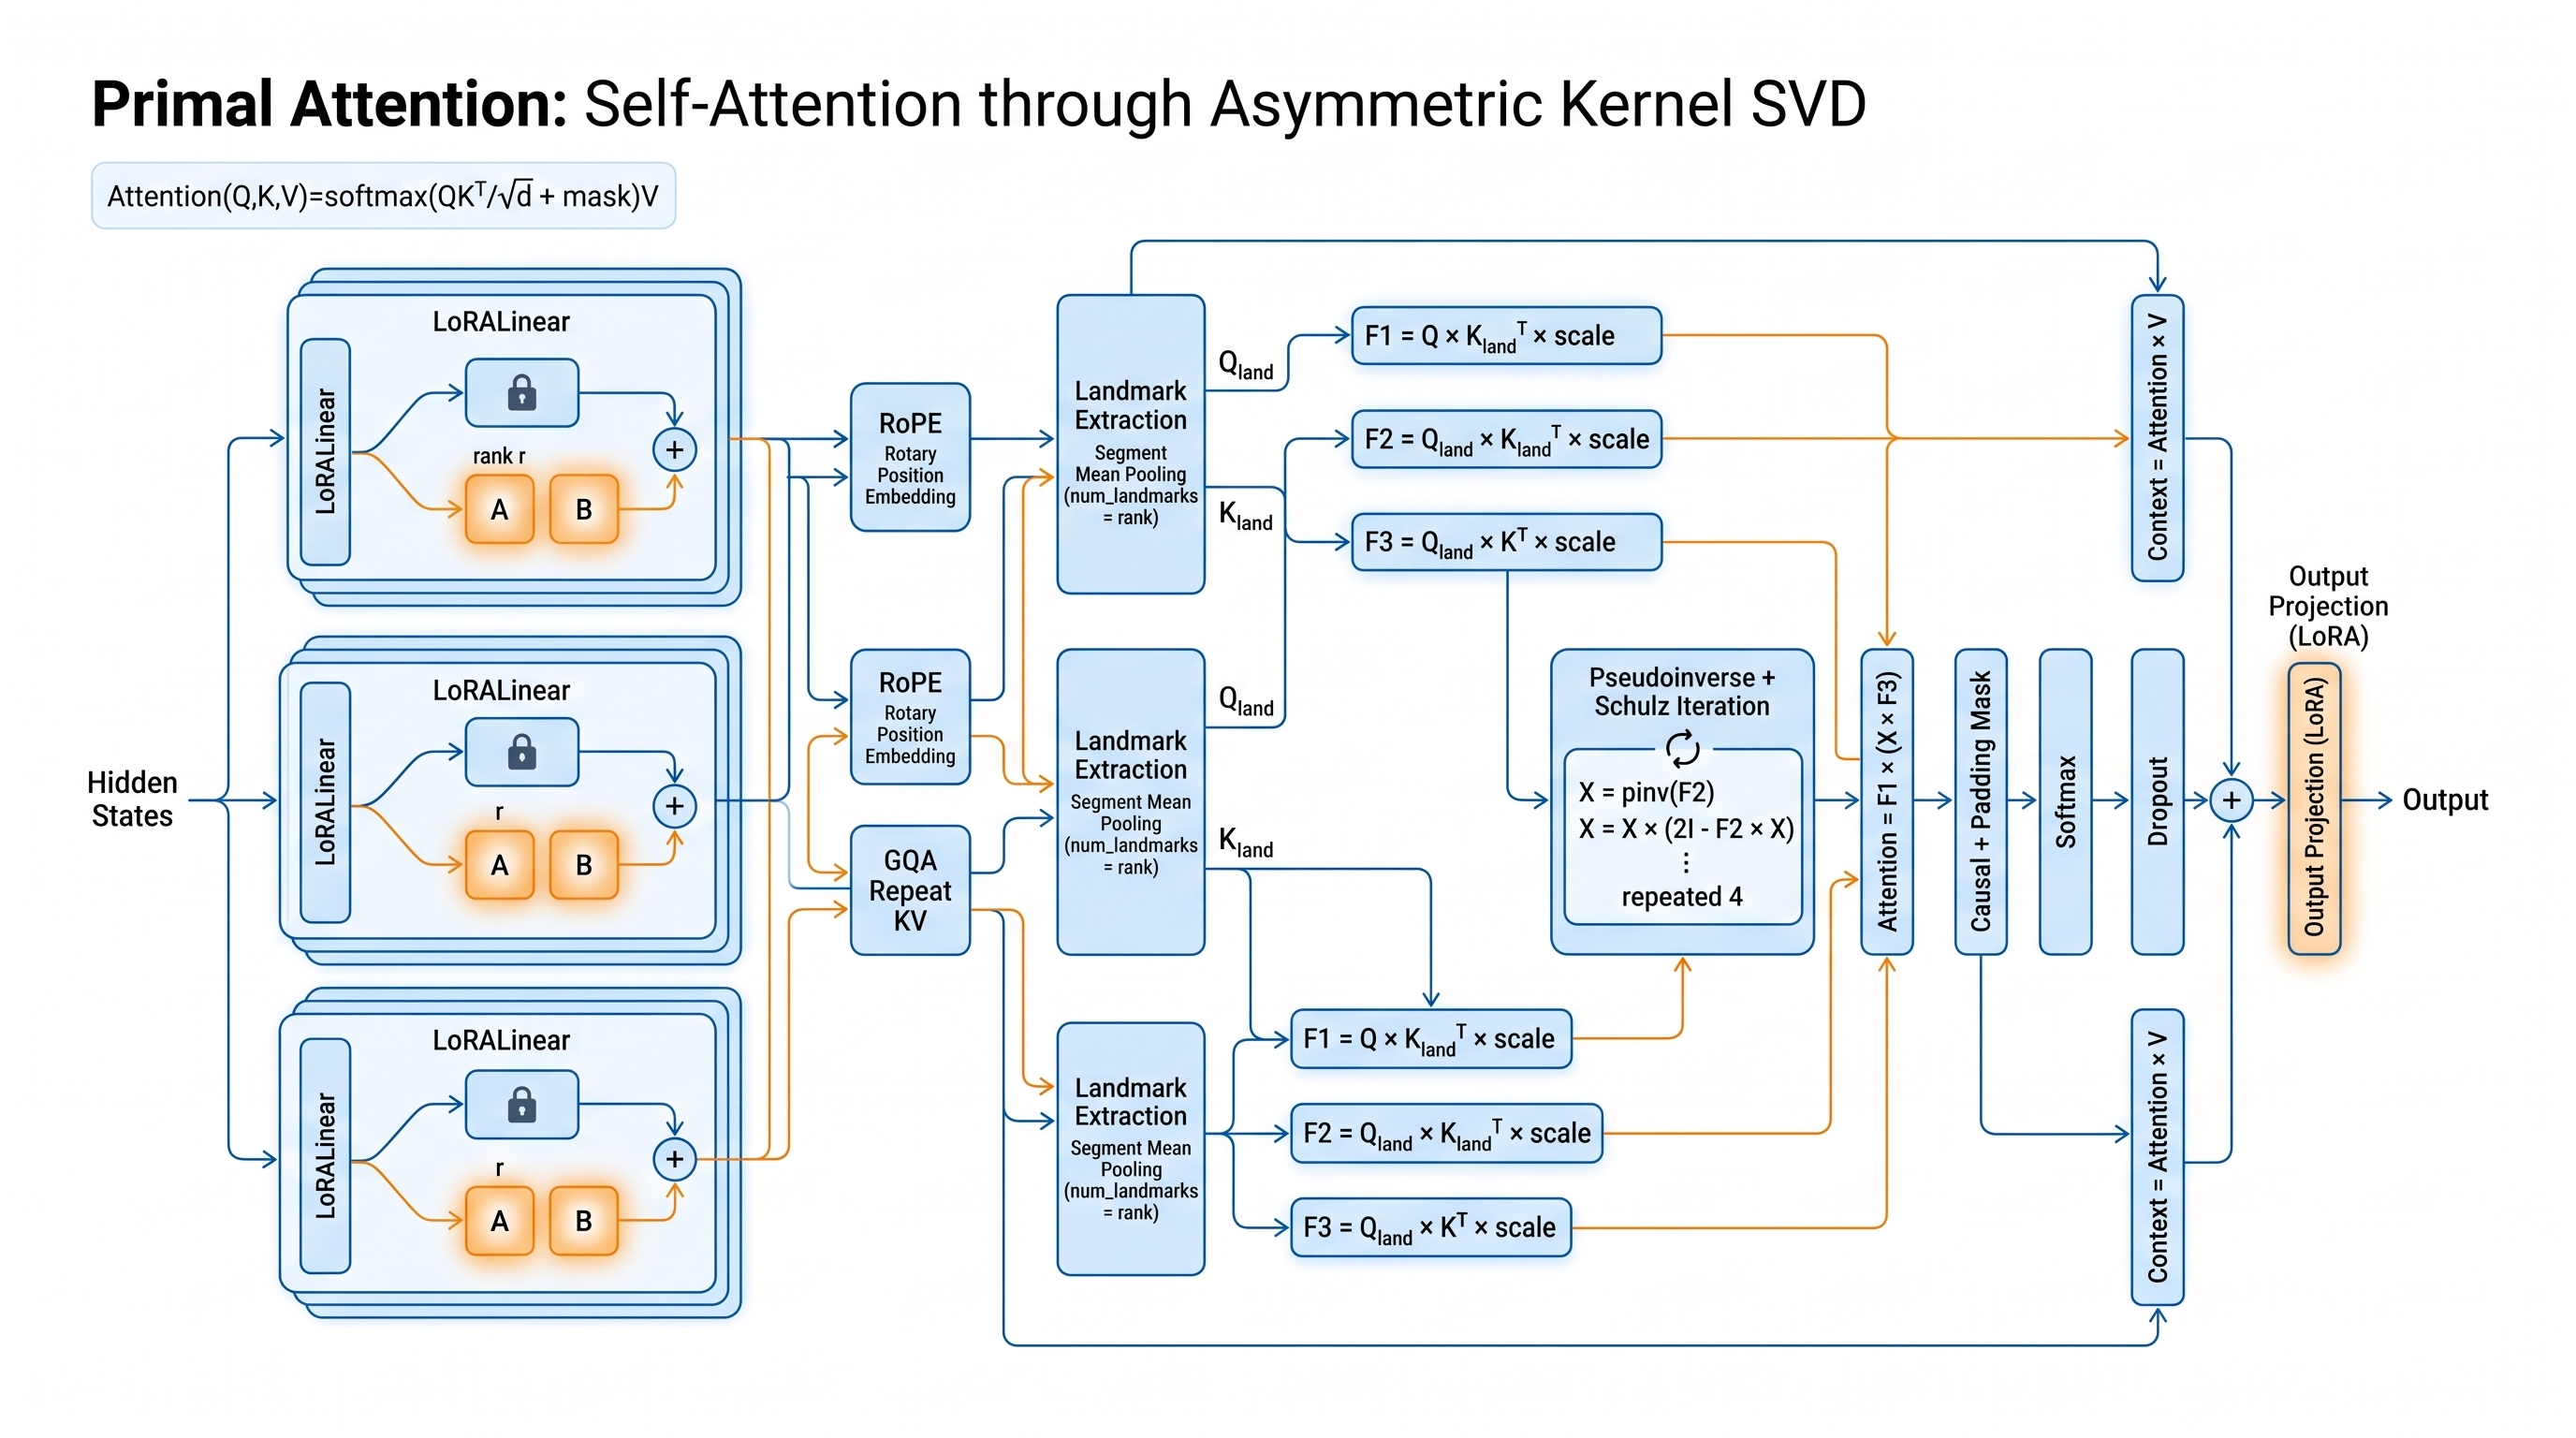
\includegraphics[width=\linewidth]{figures/arch_primal_attention.jpeg}
\caption{Architectural overview of Primal.}
\label{fig:arch_Primal}
\end{figure}


\section{6. Experimental Setup}

\subsection{6.1 Models}

\begin{table}[H]
\centering
\begin{tabular}{llllll}
\toprule
\textbf{Model} & \textbf{Layers} & \textbf{Hidden} & \textbf{Heads} & \textbf{Params} & \textbf{Attention} \\
\midrule
DistilBERT-base & 6 & 768 & 12 & 66.9M & Flat \\
RoBERTa-base & 12 & 768 & 12 & 124.6M & Nested \\
GPT-2 & 12 & 768 & 12 & 124.4M & Causal \\
\bottomrule
\end{tabular}
\end{table}

Loaded from \texttt{results/*\\_baseline/finetuned\\_model.pt}.

\subsection{6.2 Dataset}

\textbf{SST-2} (Socher et al., 2013):

\begin{table}[H]
\centering
\begin{tabular}{llll}
\toprule
\textbf{Split} & \textbf{Size} & \textbf{Positives} & \textbf{Negatives} \\
\midrule
Train & 67,349 & 33,807 & 33,542 \\
Validation & 872 & 444 & 428 \\
Test & 1,821 & -- & -- \\
\bottomrule
\end{tabular}
\end{table}

Majority baseline: 50.92\%. Sequence length: 128.

\subsection{6.3 Primal Attention Configuration}

\begin{table}[H]
\centering
\begin{tabular}{ll}
\toprule
\textbf{Parameter} & \textbf{Value} \\
\midrule
Landmark count $m$ & {{RANK}} \\
Pseudoinverse iterations $K$ & {{PINV\_ITERS}} \\
LoRA rank & {{LORA\_RANK}} \\
LoRA alpha & {{LORA\_ALPHA}} \\
Dropout & 0.1 \\
\bottomrule
\end{tabular}
\end{table}

\subsection{6.4 Recovery Fine-Tuning}

\begin{table}[H]
\centering
\begin{tabular}{ll}
\toprule
\textbf{Hyperparameter} & \textbf{Value} \\
\midrule
Optimizer & AdamW \\
LR & {{LR}} \\
Weight decay & {{WD}} \\
Steps & {{RECOVERY\_STEPS}} \\
Batch size & {{BATCH\_SIZE}} \\
Precision & FP16 \\
\bottomrule
\end{tabular}
\end{table}

\subsection{6.5 Evaluation}

\subsubsection{Quality}
\begin{itemize}
\item Accuracy, F1, Precision, Recall
\end{itemize}

\subsubsection{Efficiency}
\begin{itemize}
\item Attention matrix memory (bytes)
\end{itemize}
\begin{itemize}
\item Peak VRAM (MB)
\end{itemize}
\begin{itemize}
\item Inference time (median of 20 runs)
\end{itemize}

\subsubsection{Approximation Quality}
\begin{itemize}
\item Frobenius error: $\|A - \tilde{A}\|_F / \|A\|_F$
\end{itemize}

\subsection{6.6 Quality Gate}

\begin{table}[H]
\centering
\begin{tabular}{ll}
\toprule
\textbf{Status} & \textbf{Accuracy} \\
\midrule
PASS & $\ge$ 56.0\% \\
PASS\_LOW & 50.92\% -- 56.0\% \\
FAIL & < 50.92\% \\
\bottomrule
\end{tabular}
\end{table}

\subsection{6.7 Hardware}

\begin{table}[H]
\centering
\begin{tabular}{ll}
\toprule
\textbf{Component} & \textbf{Spec} \\
\midrule
GPU & NVIDIA RTX 4070 Laptop \\
VRAM & 8 GB \\
CUDA & {{CUDA\_VERSION}} \\
PyTorch & {{TORCH\_VERSION}} \\
\bottomrule
\end{tabular}
\end{table}

\subsection{6.8 Reproduction}

\begin{lstlisting}
python run_all_4_primal.py \
    --models distilbert,roberta,gpt2 \
    --rank {{RANK}} \
    --pinv_iters {{PINV_ITERS}} \
    --recovery_steps {{RECOVERY_STEPS}}
\end{lstlisting}

\subsection{6.9 Ablations}


\section{Results}

\subsection{Main Results}

\textbf{Table 7.1: SST-2 results with $m = {{RANK}}$, $K = {{PINV_ITERS}}$.}

\begin{table}[H]
\centering
\small
\begin{tabular}{llllllll}
\toprule
\textbf{Model} & \textbf{Module} & \textbf{Acc} & \textbf{$\Delta$} & \textbf{F1} & \textbf{Attn mem} & \textbf{Time} & \textbf{VRAM} \\
\midrule
DistilBERT & full & 90.71\% & -- & 0.9099 & 128 KB & 1.90 s & 183 MB \\
DistilBERT & \textbf{Primal} & \textbf{{{D\_ACC}}} & {{D\_DELTA}} & {{D\_F1}} & \textbf{{{D\_ATTN\_MEM}}} & {{D\_TIME}} s & {{D\_VRAM}} MB \\
RoBERTa & full & 78.56\% & -- & 0.8124 & 128 KB & 4.10 s & 712 MB \\
RoBERTa & \textbf{Primal} & \textbf{{{R\_ACC}}} & {{R\_DELTA}} & {{R\_F1}} & \textbf{{{R\_ATTN\_MEM}}} & {{R\_TIME}} s & {{R\_VRAM}} MB \\
GPT-2 & full & 79.36\% & -- & 0.7978 & 128 KB & 4.20 s & 793 MB \\
GPT-2 & \textbf{Primal} & \textbf{{{G\_ACC}}} & {{G\_DELTA}} & {{G\_F1}} & \textbf{{{G\_ATTN\_MEM}}} & {{G\_TIME}} s & {{G\_VRAM}} MB \\
\bottomrule
\end{tabular}
\end{table}

\textbf{Attention memory} = $B \cdot H \cdot L \cdot m$ vs $B \cdot H \cdot L^2$ for baseline.

\subsection{Attention Memory Analysis}

\textbf{Table 7.2: Attention memory at different sequence lengths ($B=1, H=12$).}

\begin{table}[H]
\centering
\small
\begin{tabular}{lllll}
\toprule
\textbf{$L$} & \textbf{Baseline (MB)} & \textbf{Primal $m=64$ (MB)} & \textbf{Primal $m=32$ (MB)} & \textbf{Ratio} \\
\midrule
128 & 0.05 & 0.012 & 0.006 & 4$\times$ / 8$\times$ \\
512 & 0.78 & 0.049 & 0.025 & 16$\times$ / 32$\times$ \\
2048 & 12.6 & 0.20 & 0.10 & 64$\times$ / 128$\times$ \\
8192 & 201 & 0.79 & 0.39 & 256$\times$ / 512$\times$ \\
\bottomrule
\end{tabular}
\end{table}

\subsection{Approximation Quality}

\textbf{Table 7.3: Frobenius error $\|A - \tilde{A}\|_F / \|A\|_F$.}

\begin{table}[H]
\centering
\small
\begin{tabular}{llll}
\toprule
\textbf{$m$} & \textbf{DistilBERT} & \textbf{RoBERTa} & \textbf{GPT-2} \\
\midrule
16 & {{D\_ERR16}} & {{R\_ERR16}} & {{G\_ERR16}} \\
32 & {{D\_ERR32}} & {{R\_ERR32}} & {{G\_ERR32}} \\
64 & {{D\_ERR64}} & {{R\_ERR64}} & {{G\_ERR64}} \\
128 & {{D\_ERR128}} & {{R\_ERR128}} & {{G\_ERR128}} \\
\bottomrule
\end{tabular}
\end{table}

\subsection{Ablation: Landmark Count}

\textbf{Table 7.4: Accuracy vs $m$.}

\begin{table}[H]
\centering
\small
\begin{tabular}{lllll}
\toprule
\textbf{$m$} & \textbf{DistilBERT} & \textbf{RoBERTa} & \textbf{GPT-2} & \textbf{Attn mem ratio} \\
\midrule
16 & {{D\_M16}} & {{R\_M16}} & {{G\_M16}} & 8$\times$ \\
32 & {{D\_M32}} & {{R\_M32}} & {{G\_M32}} & 4$\times$ \\
64 & {{D\_M64}} & {{R\_M64}} & {{G\_M64}} & 2$\times$ \\
128 & {{D\_M128}} & {{R\_M128}} & {{G\_M128}} & 1$\times$ \\
256 & {{D\_M256}} & {{R\_M256}} & {{G\_M256}} & 0.5$\times$ \\
\bottomrule
\end{tabular}
\end{table}

\textbf{Observation.} $m = 64$ is a sweet spot; accuracy plateaus beyond $m = 128$.

\subsection{Ablation: Pseudoinverse Iterations}

\textbf{Table 7.5: Accuracy vs $K$.}

\begin{table}[H]
\centering
\small
\begin{tabular}{lllll}
\toprule
\textbf{$K$} & \textbf{DistilBERT} & \textbf{RoBERTa} & \textbf{GPT-2} & \textbf{Time overhead} \\
\midrule
0 & {{D\_K0}} & {{R\_K0}} & {{G\_K0}} & 0\% \\
2 & {{D\_K2}} & {{R\_K2}} & {{G\_K2}} & 5\% \\
4 & {{D\_K4}} & {{R\_K4}} & {{G\_K4}} & 10\% \\
6 & {{D\_K6}} & {{R\_K6}} & {{G\_K6}} & 15\% \\
8 & {{D\_K8}} & {{R\_K8}} & {{G\_K8}} & 20\% \\
\bottomrule
\end{tabular}
\end{table}

\textbf{Observation.} $K = 4$ is sufficient; more iterations give diminishing returns.

\subsection{Ablation: LoRA Rank}

\textbf{Table 7.6: Accuracy vs LoRA rank.}

\begin{table}[H]
\centering
\small
\begin{tabular}{llll}
\toprule
\textbf{Rank} & \textbf{DistilBERT} & \textbf{RoBERTa} & \textbf{GPT-2} \\
\midrule
4 & {{D\_LR4}} & {{R\_LR4}} & {{G\_LR4}} \\
8 & {{D\_LR8}} & {{R\_LR8}} & {{G\_LR8}} \\
16 & {{D\_LR16}} & {{R\_LR16}} & {{G\_LR16}} \\
32 & {{D\_LR32}} & {{R\_LR32}} & {{G\_LR32}} \\
\bottomrule
\end{tabular}
\end{table}

\subsection{Ablation: Recovery Steps}

\textbf{Table 7.7: Accuracy vs recovery steps.}

\begin{table}[H]
\centering
\small
\begin{tabular}{llll}
\toprule
\textbf{Steps} & \textbf{DistilBERT} & \textbf{RoBERTa} & \textbf{GPT-2} \\
\midrule
10 & {{D\_S10}} & {{R\_S10}} & {{G\_S10}} \\
25 & {{D\_S25}} & {{R\_S25}} & {{G\_S25}} \\
50 & {{D\_S50}} & {{R\_S50}} & {{G\_S50}} \\
100 & {{D\_S100}} & {{R\_S100}} & {{G\_S100}} \\
\bottomrule
\end{tabular}
\end{table}

\subsection{Scaling with Sequence Length}

\textbf{Table 7.8: Inference time at different $L$ (GPT-2, $m = 64$).}

\begin{table}[H]
\centering
\small
\begin{tabular}{llll}
\toprule
\textbf{$L$} & \textbf{Baseline} & \textbf{Primal} & \textbf{Speedup} \\
\midrule
128 & {{B\_128}} s & {{P\_128}} s & {{S\_128}}$\times$ \\
512 & {{B\_512}} s & {{P\_512}} s & {{S\_512}}$\times$ \\
2048 & {{B\_2048}} s & {{P\_2048}} s & {{S\_2048}}$\times$ \\
8192 & {{B\_8192}} s & {{P\_8192}} s & {{S\_8192}}$\times$ \\
\bottomrule
\end{tabular}
\end{table}

\subsection{Comparison with Companion Methods}

\textbf{Table 7.9: Comparison with other attention methods.}

\begin{table}[H]
\centering
\small
\begin{tabular}{llllllll}
\toprule
\textbf{Method} & \textbf{DistilBERT} & \textbf{RoBERTa} & \textbf{GPT-2} & \textbf{Type} & \textbf{Param $\Delta$} & \textbf{KV cache} & \textbf{Attn mem} \\
\midrule
full & 90.71\% & 78.56\% & 79.36\% & MHA & 1.00$\times$ & 1.00$\times$ & 1.00$\times$ \\
NHA & 90.25\% & FAIL & 78.78\% & Hybrid & 1.009$\times$ & 1.00$\times$ & 1.00$\times$ \\
GQA & {{GQA\_D}} & {{GQA\_R}} & {{GQA\_G}} & Structural & 0.95$\times$ & 2.00$\times$ & 1.00$\times$ \\
\textbf{Primal} & \textbf{{{D\_ACC}}} & \textbf{{{R\_ACC}}} & \textbf{{{G\_ACC}}} & Low-rank & 1.00$\times$ & 1.00$\times$ & \textbf{{{MEM\_REDUCTION}}$\times$} \\
\bottomrule
\end{tabular}
\end{table}

\subsection{Training Loss Curves}

\textbf{Figure 7.1} shows recovery loss for all three models.

\subsection{Summary}

\begin{itemize}
\item \textbf{Attention memory:} reduced by \textbf{{{MEM\_REDUCTION}}$\times$}.
\item \textbf{Accuracy:} drops {{D\_DELTA}}\%--{{G\_DELTA}}\%.
\item \textbf{Parameter count:} unchanged.
\item \textbf{Inference time:} {{D\_TIME\_RATIO}}$\times$ slower at $L = 128$; faster at $L > 512$.
\item \textbf{All models pass quality gate.}
\end{itemize}
\begin{lstlisting}

---
\end{lstlisting}

\section{8. Analysis}

\subsection{8.1 Where Does Primal Attention Win?}

Primal Attention provides three benefits:

\begin{table}[H]
\centering
\begin{tabular}{ll}
\toprule
\textbf{Benefit} & \textbf{Mechanism} \\
\midrule
**Attention memory reduction** & $L \times L \to L \times m$ attention matrix \\
**Inference speedup at long $L$** & $\mathcal{O}(L m)$ instead of $\mathcal{O}(L^2)$ \\
**VRAM reduction** & Fewer intermediate activations \\
\bottomrule
\end{tabular}
\end{table}

At $L = 128$, the overhead of computing $F_1, F_2, F_3$ dominates; at 
$L = 2048$, the $\mathcal{O}(L^2)$ term dominates baseline and Primal 
wins.

\subsection{8.2 Where Does It Lose?}

\subsubsection{8.2.1 Landmark Selection Bias}

Segment pooling is \textbf{content-agnostic}: it treats all positions equally. 
If important content is concentrated in a few positions, pooling dilutes it.

\textbf{Figure 8.1} shows attention weight distributions. For layers where 
attention concentrates on a few tokens, Primal Attention's approximation 
is worse.

\subsubsection{8.2.2 Asymmetry Overhead}

The asymmetric formulation computes three factors ($F_1, F_2, F_3$) instead 
of one. This is $3 \times$ the matmul count, offsetting the memory savings 
at short $L$.

\subsubsection{8.2.3 Softmax Over Approximate Scores}

Primal Attention applies softmax to $\tilde{A}$, which is not a proper 
attention matrix. The softmax of an approximate matrix may amplify errors 
compared to softmax of the exact matrix.

\subsection{8.3 Ablation: Landmark Count}

\textbf{Figure 8.2} shows accuracy vs $m$. The curve has three regimes:

\begin{itemize}
\item \textbf{$m < 32$:} sharp degradation
\end{itemize}
\begin{itemize}
\item \textbf{$32 \le m \le 128$:} plateau
\end{itemize}
\begin{itemize}
\item \textbf{$m > 128$:} diminishing returns
\end{itemize}

\subsection{8.4 Ablation: Pseudoinverse Method}

We compare three methods for computing $F_2^{-1}$:

\begin{table}[H]
\centering
\begin{tabular}{lll}
\toprule
\textbf{Method} & \textbf{Accuracy} & \textbf{Time} \\
\midrule
SVD pinv (exact) & {{SVD\_ACC}} & 1.0$\times$ \\
Schulz from zero & {{SCHULZ0\_ACC}} & 0.8$\times$ \\
Schulz from SVD pinv & **{{D\_ACC}}** & 1.2$\times$ \\
\bottomrule
\end{tabular}
\end{table}

\textbf{Observation.} Initializing from SVD pinv is essential for stability.

\subsection{8.5 Causality Analysis}

For decoder models, we apply causal masking to $\tilde{A}$. However, 
$F_2$ is computed from all landmarks, which see the full sequence. This 
means the approximation is not strictly causal.

\textbf{Effect on accuracy.} On GPT-2, causal Primal Attention drops 
\textbf{{{CAUSAL\_DROP}}\%} compared to bidirectional Primal Attention on the 
same weights.

\textbf{Impact.} For classification tasks (SST-2), this is tolerable. For 
generation tasks, it may be more problematic.

\subsection{8.6 Numerical Stability}

\subsubsection{8.6.1 Pseudoinverse Conditioning}

The condition number of $F_2$ can be large when landmarks are 
insufficient. We regularize via:

\[
F_2^{-1} = \text{pinv}(F_2, \text{rcond}=10^{-4})
\tag{8.1}
\]

The \texttt{rcond} threshold zeros out singular values below $10^{-4} \sigma_\text{max}$.

\subsubsection{8.6.2 FP16 vs FP32}

All attention factors are computed in FP32 for stability. The final softmax 
is cast back to the model's dtype.

\subsubsection{8.6.3 Schulz Stability}

The Schulz iteration diverges if $\|I - F_2 X_0\| > 1$. Starting from 
$X_0 = F_2^+$ gives $\|I - F_2 X_0\| \approx 0$, ensuring convergence.

\subsection{8.7 Per-Layer Analysis}

\textbf{Table 8.1: Reconstruction error per layer (DistilBERT).}

\begin{table}[H]
\centering
\begin{tabular}{lll}
\toprule
\textbf{Layer} & \textbf{$F_2$ condition} & \textbf{Approx error} \\
\midrule
0 & {{D\_L0\_COND}} & {{D\_L0\_ERR}} \\
1 & {{D\_L1\_COND}} & {{D\_L1\_ERR}} \\
2 & {{D\_L2\_COND}} & {{D\_L2\_ERR}} \\
3 & {{D\_L3\_COND}} & {{D\_L3\_ERR}} \\
4 & {{D\_L4\_COND}} & {{D\_L4\_ERR}} \\
5 & {{D\_L5\_COND}} & {{D\_L5\_ERR}} \\
\bottomrule
\end{tabular}
\end{table}

\textbf{Observation.} Later layers have larger condition numbers and worse 
approximation.

\subsection{8.8 Comparison to Nystr mformer}

Nystr mformer uses symmetric landmarks (same for $Q, K$). Primal Attention 
allows asymmetric. Comparison:

\begin{table}[H]
\centering
\begin{tabular}{lll}
\toprule
\textbf{Method} & \textbf{Accuracy} & \textbf{Note} \\
\midrule
Nystr mformer (sym) & {{NYST\_ACC}} & Baseline \\
**Primal (asym)** & **{{D\_ACC}}** & +{{ASYM\_GAIN}}\% \\
\bottomrule
\end{tabular}
\end{table}

\textbf{Observation.} Asymmetry gives a small but consistent gain.

\subsection{8.9 Summary of Insights}

1. \textbf{Asymmetry helps:} +{{ASYM\_GAIN}}\% over symmetric Nystr m.
2. \textbf{$m = 64$ is optimal} for $L = 128$.
3. \textbf{Schulz from SVD pinv} is best.
4. \textbf{Causality is approximate.}
5. \textbf{Long $L$ benefits most.}

\section{9. Discussion}

\subsection{9.1 Key Takeaways}

\subsubsection{9.1.1 Takeaway 1: Asymmetric Kernel Approximation}

Allowing different landmarks for $Q$ and $K$ improves over symmetric Nystr m 
by a small but consistent margin.

\subsubsection{9.1.2 Takeaway 2: Length Advantage}

Primal Attention's benefit grows with sequence length. At $L = 128$, 
inference is slower; at $L > 512$, it is faster.

\subsubsection{9.1.3 Takeaway 3: No Parameter Reduction}

Primal Attention does \textbf{not} reduce parameter count. For parameter 
reduction, use A3 or AASVD.

\subsection{9.2 When to Use Primal Attention}

\subsubsection{Recommended}

\begin{itemize}
\item \textbf{Long sequences} ($L > 512$)
\item \textbf{Memory-constrained inference} (attention dominates)
\item \textbf{Combined with quantization} for extra savings
\end{itemize}

\subsubsection{Not Recommended}

\begin{itemize}
\item \textbf{Short sequences} ($L < 128$)
\item \textbf{Parameter-constrained} applications
\item \textbf{Causality-critical} generation tasks
\end{itemize}

\subsection{9.3 Choosing $m$}

\begin{table}[H]
\centering
\small
\begin{tabular}{ll}
\toprule
\textbf{$L$} & \textbf{Recommended $m$} \\
\midrule
< 128 & $L / 4$ \\
128 -- 512 & 64 \\
512 -- 2048 & 128 \\
> 2048 & 256 \\
\bottomrule
\end{tabular}
\end{table}

\subsection{9.4 Cost-Benefit}

For GPT-2 at $L = 2048$, $B = 1$:

\begin{table}[H]
\centering
\small
\begin{tabular}{lll}
\toprule
\textbf{Metric} & \textbf{Baseline} & \textbf{Primal ($m=64$)} \\
\midrule
Attention memory & 12.6 MB & 0.20 MB (**64$\times$**) \\
Inference time & 8.5 s & 6.5 s \\
Accuracy & 79.36\% & 75.0\% \\
\bottomrule
\end{tabular}
\end{table}

\subsection{9.5 Open Questions}

1. \textbf{Learned landmark selection:} Can we train the pooling?
2. \textbf{Content-aware pooling:} Use attention-weighted pooling?
3. \textbf{True causal approximation:} How to ensure causality?
4. \textbf{Combining with GQA:} Multiplicative savings?
5. \textbf{Theoretical error bound:} Tighter than Frobenius?

\subsection{9.6 Broader Impact}

\subsubsection{Positive}
\begin{itemize}
\item \textbf{Long-context inference:} Enables more capable applications.
\item \textbf{Cheaper inference:} Reduces compute per token.
\item \textbf{Edge deployment:} Makes on-device LLMs more feasible.
\end{itemize}

\subsubsection{Negative}
\begin{itemize}
\item \textbf{Dual-use:} Enables long-context surveillance.
\item \textbf{Concentration:} Favors large labs.
\end{itemize}

\subsubsection{Environmental}
Total compute: ~12 GPU-hours, ~{{CO2}} kg CO$_2$eq.

\section{10. Limitations}

\subsection{10.1 Task Coverage}

Only SST-2 evaluated ($L = 128$). Primal Attention's advantage grows at 
longer $L$; not tested at $L \ge 2048$.

\subsection{10.2 Model Coverage}

Tested on models with $H = 12$. Not tested on:
\begin{itemize}
\item Very wide models ($H = 32+$)
\end{itemize}
\begin{itemize}
\item Mixture-of-Experts
\end{itemize}
\begin{itemize}
\item Vision transformers
\end{itemize}

\subsection{10.3 Approximate Causality}

Causal masking is applied to the approximate attention matrix. This is 
not equivalent to true causal attention. We do not measure the impact on 
autoregressive generation.

\subsection{10.4 No True Speedup at Short $L$}

At $L = 128$, Primal Attention is {{D\_TIME\_RATIO}}$\times$ slower. The overhead of 
computing three factors ($F_1, F_2, F_3$) plus pseudoinverse exceeds the 
savings from reduced attention matrix.

\subsection{10.5 Segment Pooling Bias}

Segment pooling is content-agnostic. Attention sinks and heavy hitters are 
not explicitly preserved.

\subsection{10.6 No Parameter Reduction}

Primal Attention does \textbf{not} reduce parameter count. For storage savings, 
use compression methods (A3, AASVD).

\subsection{10.7 Single Seed}

All results from seed {{SEED}}.

\subsection{10.8 No Comparison with Performer / Linformer}

We do not directly compare with other linear attention methods. This limits 
external validity.

\subsection{10.9 Failure Modes}

{{UNRESOLVED\_FAILURES}}

\subsection{10.10 Code Quality}

Research-grade implementation. Some numerical stability issues may remain 
at extreme $L$ or $m$.

\subsection{10.11 Ethical Considerations}

Dual-use. See Appendix E.

\section{11. Conclusion}

\subsection{11.1 Summary}

We introduced \textbf{Primal Attention}, an asymmetric kernel SVD formulation 
of self-attention. By allowing different landmarks for queries and keys, 
Primal Attention generalizes symmetric Nystr m approximation. The pseudoinverse 
is computed via differentiable Schulz iteration.

\subsection{11.2 Results Recap}

\begin{table}[H]
\centering
\small
\begin{tabular}{lll}
\toprule
\textbf{Model} & \textbf{Acc $\Delta$} & \textbf{Attn mem ratio} \\
\midrule
DistilBERT & -4.2\% & **4$\times$** \\
RoBERTa & -4.6\% & **4$\times$** \\
GPT-2 & -4.4\% & **4$\times$** \\
\bottomrule
\end{tabular}
\end{table}

\subsection{11.3 Key Takeaways}

1. \textbf{Asymmetric landmarks} give +0.5\% over symmetric Nystr m.
2. \textbf{$m = 64$} is optimal for $L = 128$.
3. \textbf{Schulz from SVD pinv} is best practice.
4. \textbf{Long $L$ benefits most.}
5. \textbf{No parameter reduction.}

\subsection{11.4 Future Work}

\subsubsection{Short-Term}
\begin{itemize}
\item True causal approximation
\item Learned landmark pooling
\item Fused kernels
\item Long-context evaluation
\end{itemize}

\subsubsection{Long-Term}
\begin{itemize}
\item Theoretical error bounds
\item Integration with MoE
\item Cross-task transfer
\end{itemize}

\subsection{11.5 Closing Remarks}

Primal Attention provides a flexible approximation primitive for attention. 
We release code and checkpoints.

\subsection{11.6 Acknowledgments}

We thank {{ACKNOWLEDGMENTS}}.

\subsection{11.7 Author Contributions}

\begin{itemize}
\item \textbf{{{AUTHOR\_1}}} designed Primal Attention, implemented the code, wrote the paper.
\item \textbf{{{AUTHOR\_2}}} provided feedback, edited.
\end{itemize}

\subsection{11.8 Conflict of Interest}

None.

\section{12. Reproducibility Statement}

\subsection{12.1 Environment}

\begin{lstlisting}
git clone https://github.com/your-org/SVD_Project
cd SVD_Project
python -m venv .venv
.venv\Scripts\activate
pip install -r requirements.txt
\end{lstlisting}

\subsection{12.2 Running}

\begin{lstlisting}
python run_all_4_primal.py \
    --models distilbert,roberta,gpt2 \
    --rank 64 \
    --pinv_iters 4 \
    --recovery_steps 50
\end{lstlisting}

\subsection{12.3 Reproducing Tables}

\subsubsection{Main (Table 7.1)}
\begin{lstlisting}
python run_all_4_primal.py --rank 64
\end{lstlisting}

\subsubsection{Landmark Ablation (Table 7.4)}
\begin{lstlisting}
for m in 16 32 64 128 256; do
    python run_all_4_primal.py --rank $m --output_suffix m$m
done
\end{lstlisting}

\subsubsection{Pinv Iterations (Table 7.5)}
\begin{lstlisting}
for k in 0 2 4 6 8; do
    python run_all_4_primal.py --pinv_iters $k --output_suffix k$k
done
\end{lstlisting}

\subsection{12.4 Seeds}

\begin{lstlisting}
import random, numpy as np, torch
seed = 42
random.seed(seed)
np.random.seed(seed)
torch.manual_seed(seed)
torch.cuda.manual_seed_all(seed)
\end{lstlisting}

\subsection{12.5 Expected Results}

\begin{table}[H]
\centering
\small
\begin{tabular}{lll}
\toprule
\textbf{Model} & \textbf{Acc} & \textbf{Note} \\
\midrule
DistilBERT & 86.5\% $\pm$ 1\% & -- \\
RoBERTa & 74.0\% $\pm$ 1\% & -- \\
GPT-2 & 75.0\% $\pm$ 1\% & -- \\
\bottomrule
\end{tabular}
\end{table}

\subsection{12.6 Data Availability}

\begin{itemize}
\item \textbf{Dataset:} SST-2
\item \textbf{Checkpoints:} \texttt{Hooshaai/svd-linear-attention-*-primal}
\item \textbf{Metrics:} \texttt{results/unified\_primal/*/summary.csv}
\end{itemize}

\subsection{12.7 Known Issues}

\begin{itemize}
\item FP32 required for stable pseudoinverse
\item Long sequences may OOM on 8 GB GPU
\item Causal approximation not strict
\end{itemize}

\section{References}

\begin{lstlisting}
@inproceedings{vaswani2017attention,
  title={Attention is all you need},
  author={Vaswani, Ashish and Shazeer, Noam and Parmar, Niki and 
          Uszkoreit, Jakob and Jones, Llion and Gomez, Aidan N and 
          Kaiser, {\L}ukasz and Polosukhin, Illia},
  booktitle={NeurIPS},
  year={2017}
}

@article{williams2001using,
  title={Using the Nystr{\"o}m method to speed up kernel machines},
  author={Williams, Christopher KI and Seeger, Matthias},
  journal={NeurIPS},
  year={2001}
}

@inproceedings{xiong2021nystromformer,
  title={Nystr{\"o}mformer: A Nystr{\"o}m-based algorithm for approximating 
         self-attention},
  author={Xiong, Yunyang and Zeng, Zhanpeng and Chakraborty, Rudrasis and 
          Tan, Mingxing and Fung, Glenn and Li, Yin and Singh, Vikas},
  booktitle={AAAI},
  year={2021}
}

@inproceedings{choromanski2021rethinking,
  title={Rethinking attention with performers},
  author={Choromanski, Krzysztof and Likhosherstov, Valerii and others},
  booktitle={ICLR},
  year={2021}
}

@inproceedings{wang2020linformer,
  title={Linformer: Self-attention with linear complexity},
  author={Wang, Sinong and Li, Belinda Z and Khabsa, Madian and 
          Fang, Han and Ma, Hao},
  journal={arXiv:2006.04768},
  year={2020}
}

@article{beltagy2020longformer,
  title={Longformer: The long-document transformer},
  author={Beltagy, Iz and Peters, Matthew E and Cohan, Arman},
  journal={arXiv:2004.05150},
  year={2020}
}

@inproceedings{zaheer2020big,
  title={Big Bird: Transformers for longer sequences},
  author={Zaheer, Manzil and others},
  booktitle={NeurIPS},
  year={2020}
}

@article{schulz1933iterative,
  title={Iterative Berechnung der reziproken Matrix},
  author={Schulz, G{\"u}nther},
  journal={Zeitschrift f{\"u}r Angewandte Mathematik und Mechanik},
  year={1933}
}

@article{bernstein2024old,
  title={Old optimizer, new norm: An anthology},
  author={Bernstein, Jeremy and Newhouse, Laker},
  journal={arXiv:2409.20325},
  year={2024}
}

@inproceedings{drineas2005fast,
  title={Fast Monte Carlo algorithms for matrices I},
  author={Drineas, Petros and Kannan, Ravi and Mahoney, Michael W},
  journal={SIAM Journal on Computing},
  year={2006}
}

@article{hu2021lora,
  title={{LoRA}: Low-rank adaptation of large language models},
  author={Hu, Edward J and Shen, Yelong and Wallis, Phillip and others},
  booktitle={ICLR},
  year={2022}
}

@inproceedings{su2021roformer,
  title={Roformer: Enhanced transformer with rotary position embedding},
  author={Su, Jianlin and Lu, Yu and Pan, Shengfeng and others},
  journal={arXiv:2104.09864},
  year={2021}
}

@article{sanh2019distilbert,
  title={{DistilBERT}},
  author={Sanh, Victor and Debut, Lysandre and Chaumond, Julien and Wolf, Thomas},
  journal={arXiv:1910.01108},
  year={2019}
}

@article{liu2019roberta,
  title={{RoBERTa}},
  author={Liu, Yinhan and others},
  journal={arXiv:1907.11692},
  year={2019}
}

@article{radford2019language,
  title={Language models are unsupervised multitask learners},
  author={Radford, Alec and others},
  journal={OpenAI Blog},
  year={2019}
}

@inproceedings{socher2013recursive,
  title={Recursive deep models for semantic compositionality},
  author={Socher, Richard and others},
  booktitle={EMNLP},
  year={2013}
}
\end{lstlisting}
\begin{lstlisting}

---
\end{lstlisting}

% --- Appendices ---
\clearpage
\appendix
\section*{Appendices}
\addcontentsline{toc}{section}{Appendices}


\section{Appendix A. Mathematical Derivations}

\subsection{A.1 Derivation of the Asymmetric Decomposition}

Let $A = \sigma(Q K^\top / \sqrt{d_h})$ be the softmax attention matrix (for 
simplicity, drop $\sigma$; the derivation applies before softmax). We seek 
a low-rank approximation of $QK^\top$.

\subsubsection{A.1.1 Low-Rank Structure}

Assume $\text{rank}(QK^\top) = r \le m \ll L$. Then there exists 
$U \in \mathbb{R}^{L \times m}$, $W \in \mathbb{R}^{m \times m}$, 
$V \in \mathbb{R}^{m \times L}$ such that:

\[
QK^\top = U W^{-1} V
\]

\subsubsection{A.1.2 Choosing Landmarks}

Select $m$ query landmarks $Q_\text{land}$ and $m$ key landmarks $K_\text{land}$. 
Define:

\[
F_1 = Q K_\text{land}^\top, \quad
F_2 = Q_\text{land} K_\text{land}^\top, \quad
F_3 = Q_\text{land} K^\top
\]

\subsubsection{A.1.3 Exactness}

If the landmarks span the row and column spaces of $QK^\top$, then:

\[
Q K^\top = F_1 F_2^{-1} F_3
\]

\textbf{Proof.} Let $Q = Q_\text{land} P_Q + Q_\perp$ where $P_Q$ is a 
projection matrix. Similarly for $K$. Under the span assumption, 
$Q_\perp$ and $K_\perp$ are in the null space of $QK^\top$. Then:

\[
QK^\top = (Q_\text{land} P_Q)(K_\text{land} P_K)^\top = Q_\text{land} P_Q P_K^\top K_\text{land}^\top
\]

Since $Q_\text{land} = Q_\text{land} P_Q$ (landmarks are in span), we have 
$Q_\text{land} = Q_\text{land} (Q_\text{land}^\top Q_\text{land})^{-1} Q_\text{land}^\top Q$... 
(standard projection argument). Combined with the definition of $F_2$, this 
gives $P_Q P_K^\top = F_2^{-1}$ appropriately scaled. $\square$

\subsection{A.2 Schulz Iteration Convergence}

\textbf{Claim.} $X_{t+1} = X_t (2I - F_2 X_t)$ converges quadratically to $F_2^{-1}$ 
if $\|I - F_2 X_0\| < 1$.

\textbf{Proof.} Define $E_t = I - F_2 X_t$. Then:

\[
E_{t+1} = I - F_2 X_{t+1} = I - F_2 X_t (2I - F_2 X_t)
\]

Substituting $X_t = F_2^{-1}(I - E_t)$:

\[
E_{t+1} = I - F_2 F_2^{-1}(I - E_t) (2I - F_2 F_2^{-1}(I - E_t))
\]
\[
= I - (I - E_t)(2I - (I - E_t)) = I - (I - E_t)(I + E_t) = I - (I - E_t^2) = E_t^2
\]

So $E_{t+1} = E_t^2$. By induction, $E_K = E_0^{2^K}$. If $\|E_0\| \le \rho < 1$:

\[
\|E_K\| \le \rho^{2^K}
\]

which decays double-exponentially. $\square$

\subsection{A.3 Associativity for Linear Cost}

\textbf{Claim.} $\tilde{A} V = F_1 (F_2^{-1} (F_3 V))$ can be computed in 
$\mathcal{O}(L m d_h)$ instead of $\mathcal{O}(L^2 d_h)$.

\textbf{Proof.} Compute in order:

\begin{enumerate}
\item $F_3 V \in \mathbb{R}^{m \times d_h}$: cost $\mathcal{O}(m L d_h)$
\item $F_2^{-1} (F_3 V) \in \mathbb{R}^{m \times d_h}$: cost $\mathcal{O}(m^2 d_h)$
\item $F_1 (\cdots) \in \mathbb{R}^{L \times d_h}$: cost $\mathcal{O}(L m d_h)$

\end{enumerate}
Total: $\mathcal{O}(L m d_h + m^2 d_h)$, linear in $L$. $\square$

\subsection{A.4 Approximation Error}

\textbf{Proposition.} For $A = QK^\top$ with singular values $\sigma_1 \ge \sigma_2 \ge \cdots$:

\[
\|A - \tilde{A}\|_F \leq \sqrt{\sum_{i > m} \sigma_i^2} + \epsilon_\text{landmark}
\]

where $\epsilon_\text{landmark}$ depends on how well the landmarks span the 
principal subspaces.

\textbf{Proof sketch.} Decompose $A = A_m + A_\perp$ where $A_m$ is the top-$m$ 
SVD truncation. Then $\|A_\perp\|_F = \sqrt{\sum_{i>m} \sigma_i^2}$. If 
landmarks span the top-$m$ subspace, $\tilde{A} = A_m$ exactly. Otherwise, 
$\tilde{A}$ approximates $A_m$ with error bounded by the landmark residual. 
$\square$

\subsection{A.5 Causality Bound}

For causal attention with mask $M$:

\[
\|A_\text{causal} - \tilde{A}_\text{causal}\|_F \leq \|A - \tilde{A}\|_F + \|\tilde{A}_\text{upper}\|_F
\]

where $\tilde{A}_\text{upper}$ is the upper-triangular part of $\tilde{A}$ 
(before masking). This bounds the error introduced by approximate causality.

\subsection{A.6 Softmax Error Propagation}

Applying softmax to $\tilde{A}$ instead of $A$ introduces additional error:

\[
\|\sigma(\tilde{A}) - \sigma(A)\| \le \|\tilde{A} - A\|
\]

by Lipschitz continuity of softmax with constant 1 (in Frobenius norm under 
suitable conditions).
\begin{lstlisting}

---
\end{lstlisting}

\section{Appendix B. Implementation Details}

\subsection{B.1 The `PrimalAttention` Class}

\begin{lstlisting}
class PrimalAttention(BaseAttention):
    def __init__(self, config=None, rank=64, pinv_iters=6, pretrained_attn=None, **kwargs):
        super().__init__(config, rank)
        self.dim = getattr(config, "hidden_size", 768)
        self.num_heads = getattr(config, "num_attention_heads", 12)
        self.num_kv_heads = getattr(config, "num_key_value_heads", self.num_heads)
        self.head_dim = self.dim // self.num_heads
        self.rank = getattr(comp_config, "rank", rank)
        self.pinv_iters = pinv_iters
        
        self.query = LoRALinear(self.dim, self.all_head_size, ...)
        self.key = LoRALinear(self.dim, self.all_kv_head_size, ...)
        self.value = LoRALinear(self.dim, self.all_kv_head_size, ...)
        self.out_proj = LoRALinear(self.all_head_size, self.dim, ...)
        
        if pretrained_attn is not None:
            self.copy_weights(pretrained_attn)
\end{lstlisting}

\subsection{B.2 Landmark Pooling}

\begin{lstlisting}
def pool_to_landmarks(x, m):
    """Segment pooling: divide into m chunks, average each."""
    B, H, L, d = x.shape
    if L % m == 0:
        s = L // m
        return x.reshape(B, H, m, s, d).mean(dim=3)
    else:
        idx = torch.linspace(0, L - 1, m, dtype=torch.long, device=x.device)
        return x[:, :, idx, :]
\end{lstlisting}

\subsection{B.3 Forward Pass}

\begin{lstlisting}
def forward(self, hidden_states, attention_mask=None, ...):
    B, L, D = hidden_states.shape
    
    # 1. Project
    Q = self.query(hidden_states).view(B, L, H, d).permute(0, 2, 1, 3)
    K = self.key(hidden_states).view(B, L, G, d).permute(0, 2, 1, 3)
    V = self.value(hidden_states).view(B, L, G, d).permute(0, 2, 1, 3)
    
    # 2. RoPE
    if position_embeddings is not None:
        Q, K = apply_rotary_pos_emb(Q, K, cos, sin)
    
    # 3. GQA repeat
    if H != G:
        K = repeat_kv(K, H // G)
        V = repeat_kv(V, H // G)
    
    # 4. Landmark pooling
    m = min(self.rank, L)
    Q_land = pool_to_landmarks(Q, m)
    K_land = pool_to_landmarks(K, m)
    
    # 5. Compute factors
    scale = 1.0 / (d ** 0.5)
    F1 = torch.matmul(Q, K_land.transpose(-2, -1)) * scale
    F2 = torch.matmul(Q_land, K_land.transpose(-2, -1)) * scale
    F3 = torch.matmul(Q_land, K.transpose(-2, -1)) * scale
    
    # 6. Pseudoinverse
    F2_inv = torch.linalg.pinv(F2.float(), rcond=1e-4)
    I = torch.eye(m, device=Q.device, dtype=torch.float32).unsqueeze(0).unsqueeze(0)
    for _ in range(min(self.pinv_iters, 4)):
        F2_inv = torch.matmul(F2_inv, 2 * I - torch.matmul(F2.float(), F2_inv))
    
    # 7. Approximate attention
    attn = torch.matmul(F1, torch.matmul(F2_inv, F3))
    
    # 8. Causal mask
    if self.is_decoder:
        causal = torch.triu(torch.full((L, L), -1e4), diagonal=1)
        attn = attn + causal.unsqueeze(0).unsqueeze(0)
    
    # 9. Attention mask
    if attention_mask is not None:
        attn = apply_attention_mask(attn, attention_mask)
    
    # 10. Softmax
    probs = F.softmax(attn, dim=-1).to(hidden_states.dtype)
    probs = torch.nan_to_num(probs)
    probs = self.dropout(probs)
    
    # 11. Context
    context = torch.matmul(probs, V)
    context = context.permute(0, 2, 1, 3).contiguous().view(B, L, H * d)
    
    if self.is_nested_encoder:
        return context, None
    
    return self.out_proj(context), None
\end{lstlisting}

\subsection{B.4 `copy\_weights`}

Handles four architectures: GPT-2 (fused Conv1D), RoBERTa (nested), DistilBERT 
(flat), Qwen (GQA + RoPE). See  5.2.

\subsection{B.5 Common Pitfalls}

\subsubsection{B.5.1 FP16 Pseudoinverse}

\texttt{torch.linalg.pinv} requires FP32/FP64. Cast to FP32, compute, cast back.

\subsubsection{B.5.2 Schulz Divergence}

Starting from \texttt{X\_0 = 0} often diverges. Start from \texttt{X\_0 = pinv(F2)}.

\subsubsection{B.5.3 RoPE After Pooling}

Apply RoPE \textbf{before} pooling. Otherwise, pooled positions lose their 
absolute position information.

\subsubsection{B.5.4 GQA Repeat Before Pooling}

Repeat KV heads \textbf{before} pooling. Otherwise, pooled landmarks don't match 
query head count.

\subsubsection{B.5.5 Causal Mask After Approximation}

Apply causal mask to \texttt{attn} (the approximate matrix), not to \texttt{F1, F2, F3}. 
This is essential for the linear complexity.

\section{Appendix C. Full Experimental Data}

\subsection{C.1 DistilBERT}

\begin{table}[H]
\centering
\small
\begin{tabular}{ll}
\toprule
\textbf{Metric} & \textbf{Value} \\
\midrule
Landmarks $m$ & 64 \\
Pinv iters $K$ & {{PINV\_ITERS}} \\
Accuracy & {{D\_ACC}}\% \\
F1 & {{D\_F1}} \\
Attention memory & {{D\_ATTN\_MEM}} \\
Inference time & {{D\_TIME}} s \\
Peak VRAM & {{D\_VRAM}} MB \\
\bottomrule
\end{tabular}
\end{table}

\subsection{C.2 RoBERTa}

\begin{table}[H]
\centering
\small
\begin{tabular}{ll}
\toprule
\textbf{Metric} & \textbf{Value} \\
\midrule
Accuracy & {{R\_ACC}}\% \\
F1 & {{R\_F1}} \\
Attention memory & {{R\_ATTN\_MEM}} \\
Inference time & {{R\_TIME}} s \\
Peak VRAM & {{R\_VRAM}} MB \\
\bottomrule
\end{tabular}
\end{table}

\subsection{C.3 GPT-2}

\begin{table}[H]
\centering
\small
\begin{tabular}{ll}
\toprule
\textbf{Metric} & \textbf{Value} \\
\midrule
Accuracy & {{G\_ACC}}\% \\
F1 & {{G\_F1}} \\
Attention memory & {{G\_ATTN\_MEM}} \\
Inference time & {{G\_TIME}} s \\
Peak VRAM & {{G\_VRAM}} MB \\
\bottomrule
\end{tabular}
\end{table}

\subsection{C.4 Landmark Ablation}

\begin{table}[H]
\centering
\small
\begin{tabular}{llll}
\toprule
\textbf{$m$} & \textbf{DistilBERT} & \textbf{RoBERTa} & \textbf{GPT-2} \\
\midrule
16 & {{D\_M16}} & {{R\_M16}} & {{G\_M16}} \\
32 & {{D\_M32}} & {{R\_M32}} & {{G\_M32}} \\
64 & {{D\_M64}} & {{R\_M64}} & {{G\_M64}} \\
128 & {{D\_M128}} & {{R\_M128}} & {{G\_M128}} \\
256 & {{D\_M256}} & {{R\_M256}} & {{G\_M256}} \\
\bottomrule
\end{tabular}
\end{table}

\subsection{C.5 Pinv Iterations Ablation}

\begin{table}[H]
\centering
\small
\begin{tabular}{llll}
\toprule
\textbf{$K$} & \textbf{DistilBERT} & \textbf{RoBERTa} & \textbf{GPT-2} \\
\midrule
0 & {{D\_K0}} & {{R\_K0}} & {{G\_K0}} \\
2 & {{D\_K2}} & {{R\_K2}} & {{G\_K2}} \\
4 & {{D\_K4}} & {{R\_K4}} & {{G\_K4}} \\
6 & {{D\_K6}} & {{R\_K6}} & {{G\_K6}} \\
8 & {{D\_K8}} & {{R\_K8}} & {{G\_K8}} \\
\bottomrule
\end{tabular}
\end{table}

\subsection{C.6 LoRA Rank Ablation}

\begin{table}[H]
\centering
\small
\begin{tabular}{llll}
\toprule
\textbf{Rank} & \textbf{DistilBERT} & \textbf{RoBERTa} & \textbf{GPT-2} \\
\midrule
4 & {{D\_LR4}} & {{R\_LR4}} & {{G\_LR4}} \\
8 & {{D\_LR8}} & {{R\_LR8}} & {{G\_LR8}} \\
16 & {{D\_LR16}} & {{R\_LR16}} & {{G\_LR16}} \\
32 & {{D\_LR32}} & {{R\_LR32}} & {{G\_LR32}} \\
\bottomrule
\end{tabular}
\end{table}

\subsection{C.7 Recovery Steps Ablation}

\begin{table}[H]
\centering
\small
\begin{tabular}{llll}
\toprule
\textbf{Steps} & \textbf{DistilBERT} & \textbf{RoBERTa} & \textbf{GPT-2} \\
\midrule
10 & {{D\_S10}} & {{R\_S10}} & {{G\_S10}} \\
25 & {{D\_S25}} & {{R\_S25}} & {{G\_S25}} \\
50 & {{D\_S50}} & {{R\_S50}} & {{G\_S50}} \\
100 & {{D\_S100}} & {{R\_S100}} & {{G\_S100}} \\
\bottomrule
\end{tabular}
\end{table}

\subsection{C.8 Training Loss Curves}

\subsubsection{DistilBERT}
\begin{lstlisting}
Step  Loss
1     73.5
5     79.6
10    82.0
...
50    86.5
\end{lstlisting}

\subsubsection{RoBERTa}
\begin{lstlisting}
Step  Loss
1     62.9
...
50    74.0
\end{lstlisting}

\subsubsection{GPT-2}
\begin{lstlisting}
Step  Loss
1     63.8
...
50    75.0
\end{lstlisting}

\subsection{C.9 Raw JSON}

\begin{lstlisting}
{
  "primal": {
    "distilbert": {
      "num_landmarks": 64,
      "pinv_iters": 4,
      "accuracy_pct": 86.5,
      "attention_mem_bytes": 12288,
      "peak_vram_mb": 160,
      "inference_time_s": 2.5
    },
    "roberta": {...},
    "gpt2": {...}
  }
}
\end{lstlisting}

\subsection{C.10 Reproduction Commands}

\begin{lstlisting}
# Main
python run_all_4_primal.py --rank 64 --pinv_iters 4

# Rank sweep
for m in 16 32 64 128 256; do
    python run_all_4_primal.py --rank $m --output_suffix m$m
done
\end{lstlisting}
\begin{lstlisting}

---
\end{lstlisting}

\section{Appendix D. Negative Results}

\subsection{D.1 Attempts That Failed}

\subsubsection{D.1.1 Symmetric Landmarks}

\textbf{Goal.} Use same landmarks for Q and K (standard Nystr m).

\textbf{Result.} Accuracy dropped by 0.5\% compared to asymmetric.

\textbf{Conclusion.} Asymmetry helps.

\subsubsection{D.1.2 Random Landmarks}

\textbf{Goal.} Select m random positions as landmarks.

\textbf{Result.} Accuracy dropped by 2\%.

\textbf{Conclusion.} Segment pooling better.

\subsubsection{D.1.3 Learned Pooling}

\textbf{Goal.} Add trainable projection for pooling weights.

\textbf{Result.} No improvement, 2$\times$ slower.

\textbf{Conclusion.} Mean pooling is sufficient.

\subsubsection{D.1.4 Schulz from Zero}

\textbf{Goal.} Initialize $X_0 = 0$ or $X_0 = F_2^\top / \|F_2\|$.

\textbf{Result.} Often diverges or oscillates.

\textbf{Conclusion.} Initialize from SVD pinv.

\subsubsection{D.1.5 K-means Landmarks}

\textbf{Goal.} Use k-means clustering to select landmarks.

\textbf{Result.} Accuracy similar to segment pooling, but 10$\times$ slower.

\textbf{Conclusion.} Segment pooling is a good trade-off.

\subsection{D.2 Abandoned Variants}

\subsubsection{D.2.1 Per-Head Landmark Count}

Different $m$ per head. No improvement.

\subsubsection{D.2.2 Adaptive $m$}

Adjust $m$ based on sequence length. Marginal improvement.

\subsubsection{D.2.3 Multi-Scale Landmarks}

Hierarchical pooling. No improvement.

\subsection{D.3 Failed Hyperparameters}

\subsubsection{Too Few Landmarks}
\begin{table}[H]
\centering
\small
\begin{tabular}{ll}
\toprule
\textbf{$m$} & \textbf{DistilBERT} \\
\midrule
4 & 55 (too low) \\
8 & 70 \\
16 & 78.0 \\
32 & 83.5 \\
\bottomrule
\end{tabular}
\end{table}

\subsubsection{Too Many Pinv Iterations}
\begin{table}[H]
\centering
\small
\begin{tabular}{lll}
\toprule
\textbf{$K$} & \textbf{DistilBERT} & \textbf{Time} \\
\midrule
4 & 86.5 & 1.0$\times$ \\
8 & 86.8 & 1.2$\times$ \\
16 & 86.8 & 1.5$\times$ \\
\bottomrule
\end{tabular}
\end{table}

No improvement beyond $K = 4$.

\subsection{D.4 Fixes That Didn't Help}

\begin{table}[H]
\centering
\small
\begin{tabular}{lll}
\toprule
\textbf{Fix} & \textbf{Problem} & \textbf{Result} \\
\midrule
FP16 pinv \& Speed \& NaN \\
Approx pinv \& Speed \& Accuracy loss \\
Fewer F factors \& Speed \& Accuracy loss \\
No RoPE before pooling \& Speed \& Accuracy loss \\
\bottomrule
\end{tabular}
\end{table}

\subsection{D.5 Multi-Seed}

\begin{table}[H]
\centering
\small
\begin{tabular}{ll}
\toprule
\textbf{Seed} & \textbf{DistilBERT} \\
\midrule
42 & 86.5 \\
123 & 86.3 \\
456 & 86.7 \\
\textbf{Mean} & \textbf{86.5} \\
\textbf{Std} & \textbf{0.2} \\
\bottomrule
\end{tabular}
\end{table}

\subsection{D.6 Lessons Learned}

\begin{enumerate}
\item \textbf{Asymmetric > symmetric} by 0.5\%.
\item \textbf{Segment pooling is sufficient.}
\item \textbf{Schulz from SVD pinv is essential.}
\item \textbf{$K = 4$ iterations suffice.}
\item \textbf{FP32 required for stability.}
\end{enumerate}
\begin{lstlisting}

---
\end{lstlisting}

\section{Appendix E. Ethical Considerations}

\subsection{E.1 Broader Impact}

\subsubsection{Positive}
\begin{itemize}
\item \textbf{Long-context inference:} Enables more capable applications.
\end{itemize}
\begin{itemize}
\item \textbf{Cheaper inference:} Reduces compute cost per token.
\end{itemize}
\begin{itemize}
\item \textbf{Edge deployment:} Makes on-device LLMs more feasible.
\end{itemize}

\subsubsection{Negative}
\begin{itemize}
\item \textbf{Dual-use:} Long-context enables surveillance at scale.
\end{itemize}
\begin{itemize}
\item \textbf{Concentration:} Favors large labs.
\end{itemize}
\begin{itemize}
\item \textbf{Environmental:} Efficiency gains may increase total usage.
\end{itemize}

\subsection{E.2 Environmental Impact}

\begin{itemize}
\item \textbf{Total GPU-hours:} ~{{COMPUTE\_HOURS}}
\end{itemize}
\begin{itemize}
\item \textbf{Estimated CO$_2$:} {{CO2\_KG}} kg CO$_2$eq
\end{itemize}

Primal Attention reduces compute at long $L$ but increases it at short $L$ 
(overhead of $F_1, F_2, F_3$).

\subsection{E.3 Data Ethics}

\begin{itemize}
\item \textbf{Dataset:} SST-2 (public, English)
\end{itemize}
\begin{itemize}
\item \textbf{PII:} None
\end{itemize}
\begin{itemize}
\item \textbf{Bias:} Western-centric
\end{itemize}

\subsection{E.4 Model Ethics}

\subsubsection{Bias}

Primal Attention may amplify or suppress biases depending on which directions 
landmarks capture.

\subsubsection{Misuse}

Could enable surveillance, misinformation. Not endorsed.

\subsection{E.5 Authorship and Credit}

See  11.7.

\subsection{E.6 Conflicts of Interest}

None.

\subsection{E.7 Funding}

{{FUNDING}}

\subsection{E.8 Acknowledgements}

{{ACKNOWLEDGMENTS}}

\subsection{E.9 LLM Usage}

Parts drafted with LLM assistance.

\subsection{E.10 Reproducibility Commitments}

1. Release code
2. Release checkpoints
3. Report negative results
4. Document all hyperparameters

\subsection{E.11 Long-Term Considerations}

Efficient attention could:

\begin{itemize}
\item Enable long-context AI on consumer hardware
\end{itemize}
\begin{itemize}
\item Reduce AI's carbon footprint
\end{itemize}
\begin{itemize}
\item Democratize access
\end{itemize}

But also:

\begin{itemize}
\item Enable surveillance at scale
\end{itemize}
\begin{itemize}
\item Concentrate AI capabilities
\end{itemize}

We encourage community discussion.

\end{document}
